\documentclass[11pt]{article}
\usepackage{geometry}
\usepackage[utf8]{inputenc}
\usepackage[english]{babel}
\usepackage{amsmath}
\usepackage{amssymb}
\usepackage{amsfonts}
\usepackage[parfill]{parskip}
\usepackage[
    pdftex, 
    dvipsnames
]{xcolor}
\usepackage[
    colorlinks=true,
    linkcolor=black,
    urlcolor=Thistle
]{hyperref}
\usepackage{fancyhdr}
\usepackage{datetime}
\usepackage{xargs}
\usepackage{ccicons}
\usepackage{mdframed}
\usepackage{caption}
\usepackage{cancel}
\usepackage[nottoc]{tocbibind}
%\usepackage[
%    outputdir=.texpadtmp
%]{minted}
%for windows compatibility
\usepackage{float}

% ==== License =====
\usepackage[
    type={CC}, 
    modifier={by-nc-sa}, 
    version={4.0},
]{doclicense}

% ==== todo notes ====
\usepackage[
    colorinlistoftodos,
    prependcaption,
    textsize=tiny
]{todonotes}
\newcommandx{\note}[2][1=]{\todo[linecolor=Thistle,backgroundcolor=Thistle!25,bordercolor=Thistle,#1]{#2}}
\newcommandx{\unsure}[2][1=]{\todo[linecolor=red,backgroundcolor=red!25,bordercolor=red,#1]{#2}}
\newcommandx{\change}[2][1=]{\todo[linecolor=blue,backgroundcolor=blue!25,bordercolor=blue,#1]{#2}}
\newcommandx{\info}[2][1=]{\todo[linecolor=OliveGreen,backgroundcolor=OliveGreen!25,bordercolor=OliveGreen,#1]{#2}}

% General
\newcommand{\mc}[1]{\mathcal{#1}}

% Math Bold Font, Vector Notations
\newcommand{\ba}{\mathbf{a}}
\newcommand{\bb}{\mathbf{b}}
\newcommand{\bc}{\mathbf{c}}
\newcommand{\bd}{\mathbf{d}}
\newcommand{\be}{\mathbf{e}}
\renewcommand{\bf}{\mathbf{f}}
\newcommand{\bg}{\mathbf{g}}
\newcommand{\bh}{\mathbf{h}}
\newcommand{\bi}{\mathbf{i}}
\newcommand{\bj}{\mathbf{j}}
\newcommand{\bk}{\mathbf{k}}
\newcommand{\bl}{\mathbf{l}}
\newcommand{\bm}{\mathbf{m}}
\newcommand{\bn}{\mathbf{n}}
\newcommand{\bo}{\mathbf{o}}
\newcommand{\bp}{\mathbf{p}}
\newcommand{\bq}{\mathbf{q}}
\newcommand{\br}{\mathbf{r}}
\newcommand{\bs}{\mathbf{s}}
\newcommand{\bt}{\mathbf{t}}
\newcommand{\bu}{\mathbf{u}}
\newcommand{\bv}{\mathbf{v}}
\newcommand{\bw}{\mathbf{w}}
\newcommand{\bx}{\mathbf{x}}
\newcommand{\by}{\mathbf{y}}
\newcommand{\bz}{\mathbf{z}}
\newcommand{\bzero}{\mathbf{0}}

% Proofs, Structures
\newcommand{\proof}{\tit{\underline{Proof:}}} % This equivalent to the \begin{proof}\end{proof} block
\newcommand{\proofforward}{\tit{\underline{Proof($\implies$):}}}
\newcommand{\proofback}{\tit{\underline{Proof($\impliedby$):}}}
\newcommand{\proofsuperset}{\tit{\underline{Proof($\supseteq$):}}}
\newcommand{\proofsubset}{\tit{\underline{Proof($\subseteq$):}}}
\newcommand{\contradiction}{$\longrightarrow\!\longleftarrow$}
\newcommand{\qed}{\hfill $\blacksquare$}

% Number Spaces, Vector Space
\newcommand{\R}{\mathbb{R}}
\newcommand{\real}{\mathbb{R}}
\newcommand{\complex}{\mathbb{C}}
\newcommand{\field}{\mathbb{F}}

% customized commands
\newcommand{\settag}[1]{\renewcommand{\theenumi}{#1}}
\newcommand{\tbf}[1]{\textbf{#1}}
\newcommand{\tit}[1]{\textit{#1}}
\newcommand{\overbar}[1]{\mkern 1.5mu\overline{\mkern-1.5mu#1\mkern-1.5mu}\mkern 1.5mu}
\newcommand{\double}[1]{\mathbb{#1}} % Set to behave like that on word
\newcommand{\trans}[3]{$#1:#2\rightarrow{}#3$}
\newcommand{\map}[3]{\text{$\left[#1\right]_{#2}^{#3}$}}
\newcommand{\dime}[1]{\mathrm{dim}(#1)}
\newcommand{\mat}[2]{M_{#1 \times #2}(\R)}
\newcommand{\aug}{\fboxsep=-\fboxrule\!\!\!\fbox{\strut}\!\!\!}
\newcommand{\basecase}{\textsc{\underline{Basis Case:}} }
\newcommand{\inductive}{\textsc{\underline{Inductive Step:}} }
\newcommand{\norm}[1]{\left\lVert#1\right\rVert}
\newcommand{\independent}{\perp \!\!\! \perp}

% Set section number in front of equation enumerations
\counterwithin{equation}{section}
\counterwithin{footnote}{section}
\author{\ccLogo \,\,Tingfeng Xia}
\title{\textsc{CS420 Image Understanding}}
\date{Fall Term, 2020}

\begin{document}
\maketitle
\doclicenseThis
\section*{Information}
\begin{itemize}
	\item Syllabus can be found through \href{https://q.utoronto.ca/courses/181228/files/8680178/preview}{this link. }
	\item There will be office hours every weekday. :D
\end{itemize}
\tableofcontents
\newpage
\section{Linear Filter}
\subsection{Fourier Transform Overview}
\subsubsection{Sinusoidal Waves\label{sec:sinwaves}}
Consider a sinusoidal wave, it has a general form of
\begin{equation}
	A\cos \left( \omega t - \phi \right)
\end{equation}
where $A$ is the amplitude, $\omega = 2\pi f$, where $f$ is the frequency, and $\phi$ is called phase. Phase describes the horizontal shifting for the wave away from the standard position. 

\subsubsection{Vector Forms}
Consider a vector $\bv = \left( 3, 2 \right)^\top$, we write it as 
\begin{equation}
	\bv = 3\bi + 2\bj = (\bv \cdot \bi) \bi + (\bv \cdot \bj) \bj
\end{equation}
and we call $\left\{ \bi, \bj \right\}$ an orthonormal basis\footnote{$\norm{\bi} = \norm{\bj} = 1 \wedge \bi \cdot \bj = 0$}. 

\subsubsection{Inner Product on Functions Space}
Function space is an inner product space, and we can define, for a set of parametric function, on an interval of $[a, b]$ that 
\begin{equation}
	\langle f(t), g(t) \rangle = \int_a^b f(t)g(t) \,\mathrm{d} t
\end{equation}

\subsubsection{General Form (Periodic Function) - Fourier Series}
For a function $f(t)$ that is periodic with period of $T$, the general form can ben written as 
\begin{align}
	f(t) 
	&= \frac{a_0}{2} + \sum_{k = 1}^\infty a_k \cos\left(\frac{2\pi k t}{T}\right) + \sum_{k = 1}^\infty b_k \sin\left(\frac{2\pi k t}{T}\right) \\
	&= \frac{a_0}{2} \sum_{k = 1}^\infty A_k \cos\left(\frac{2\pi kt}{T} - \phi_k\right)
\end{align}
where in the second form, we merged all the sin and cos terms with the introduction of a phase term. In particular, this now takes the same form as discussed in Section \ref{sec:sinwaves}. 

\subsubsection{General Form}
The general form also takes into consideration of non-periodic functions. In such case, we need to change the summation into a integral. For any function $f(t)$, we have
\begin{equation}
	F(\omega) = \int f(t) e^{-i\omega t} \mathrm d t
\end{equation}

\subsection{Image Representation}
\subsubsection{Image}
Image is a matrix with integer values. The matrix would typically be denoted as $I$, and $I_{i, j}$ is called the \textit{\textbf{intensity}}. For each pixel, we usually represent it use an unsigned 8 bit unsigned integer and thus have range $2^0 = 0$ to $2^8 - 1 = 255$. For High Dynamic Range (HDR) images, they will be represented with 16 bit unsigned integer. Also there are cases that we (linearly) normalize the values by squashing them into $[0, 1]$. 

\subsubsection{Image Coordinates}
Image coordinates start from the top left. For a coordinate $(i, j)$, $i$ specifies that it is in the $i$-th row, and $j$ specifies column. Also worth noticing that the most upper left pixel has coordinates $(1, 1)$. 

\subsubsection{Coloured Images}
In grey scale images mentioned in the previous two parts, for a image of size $m \times n$, we have a matrix of $m \times n$ 8-bit unsigned integers. Now with the introduction of colours, we will have a tensor of $m \times n \times 3$ 8-bit ints, corresponding to three colour channels. By convention, they usually goes in the order of $R \rightarrow G \rightarrow B$. For example, $I(2, 3, 1)$ means the intensity of \textit{\textbf{red}} channel of the image at location row 2 and column 3. 

\subsubsection{Image Transformations}
For simplicity, we start with grey scale images. We can view any image as a function $f: \real^2 \rightharpoonup \mathbb{Z}_{0 - 255}$, and this enables us to transform images. An easy example would be to increase the brightness of the image, which we can achieve so with
\begin{equation}
	J(i, j)= \min \left\{ I(i, j)+\text{amount}, 255\right\}
\end{equation}
capping the max intensity at 255. Importantly, we can so some interesting operations by treating images as functions. Namely, correlation and convolution. 

\subsection{Noise Reduction}
\subsubsection{1-D Example}
Consider a signal, which is a real to real function, and our goal is to smooth the function by imposing human knowledge that the signal should be smooth and should not contain too many jitter. We can have
\begin{itemize}
	\item \textbf{Moving Average Filter}, which is $[1, ..., 1]/n$, or
	\item \textbf{Non-uniform Weights}, for example $[1, 4, 6, 4, 1] / 16$
\end{itemize}

\subsubsection{2-D Case}

\begin{figure}[H]
	\center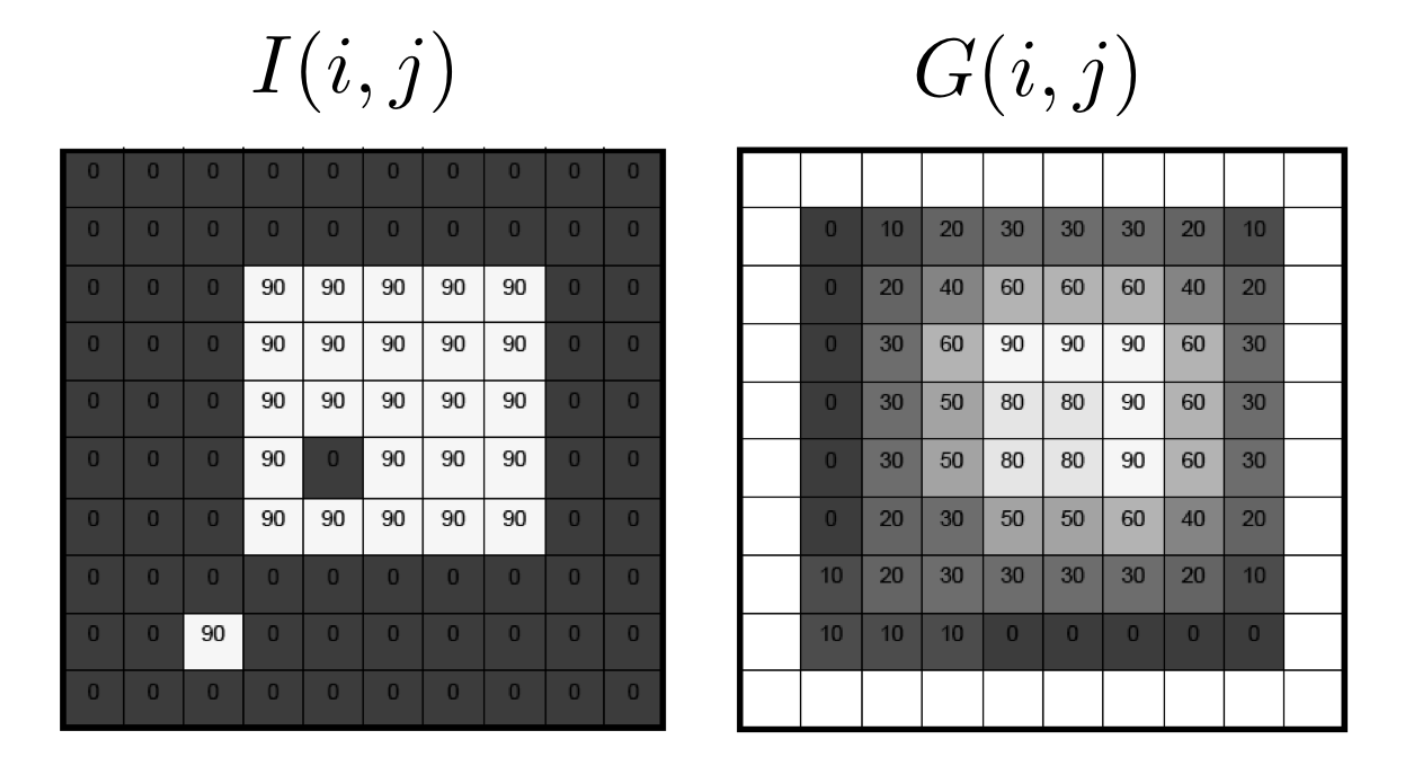
\includegraphics[width=0.6\textwidth]{figs/2dmovingaverage}
	\caption{Example of using moving average to smooth out an image, \textit{assuming no padding}. }
	\label{fig:2dmovingaverage}
\end{figure} 

Much similar to the 1-D case mentioned above, we have our choice of whether to choose an uniform filter or not. 
\begin{itemize}
	\item In the case of uniform (aka moving average), we choose (example of $3 \times 3$ filter)
		\begin{equation}
			\begin{bmatrix}
				1 & 1 & 1 \\
				1 & 1 & 1 \\
				1 & 1 & 1
			\end{bmatrix} / 9
		\end{equation}
	Figure \ref{fig:2dmovingaverage} is an example of using moving average to smooth out an image, \textit{assuming no padding}. Notice that the sharp boundaries that we used to have between dark and white is now smooth. Also, the isolated pixels ($(6, 5)$ and $(9, 3)$) are now blended in. \info{De-noising is usually an important first step (preprocessing) in any image task} 
	\item In case of non-uniform, we can again choose a gaussian like filter, such as
		\begin{equation}
			\begin{bmatrix}
				1 & 4 & 1 \\
				4 & 10 & 4 \\
				1 & 4 & 1
			\end{bmatrix} / 30
		\end{equation}
\end{itemize}

\subsection{Correlation Defined}
\subsubsection{General Moving Average}
In the general case, our filter could be any size. In particular, it needs to be of size square of an odd number. Then, the moving average becomes
\begin{equation}
	G(i, j)=\frac{1}{(2 k+1)^{2}} \sum_{u=-k}^{k} \sum_{v=-k}^{k} I(i+u, j+v)\label{eq:generalmovingaverage}
\end{equation}
\subsubsection{General Filtering}
If we apply some filter (i.e., not just a average) then we can use
\begin{equation}
	G(i, j)=\sum_{u=-k}^{k} \sum_{v=-k}^{k} F(u, v) \cdot I(i+u, j+v)\label{eq:generalfiltering}
\end{equation}
where $F(\cdot, \cdot): \real^2 \rightarrow \real$ is the called \textit{\textbf{kernel}} or \textit{\textbf{mask}} or \textit{\textbf{filter}} such that $\sum_{u'}\sum_{v'}F(u, v) = 1$. The elements of the filter is called \textit{\textbf{filter coefficients}}. Notice that if we take ($|V|, |U|$ here denotes the max values that $v, u$ can take)
\begin{equation}
	F(u, v) = \frac{1}{(2|U| + 1)^{2}} = \frac{1}{(2|V| + 1)^{2}}
\end{equation}
then Equation \ref{eq:generalfiltering} just collapses to Equation \ref{eq:generalmovingaverage}.
\subsubsection{Notation}
The Filtering operation defined above is called \textit{correlation}, denoted as
\begin{equation}
	G = F\otimes I
\end{equation}
where $F$ is our filter / kernel / mask, and $I$ is the original image. \info{Notice that filter is also an image, so $\otimes$ essentially takes two images as input and outputs one image. }

\subsubsection{Correlation - Vector Form}
Define 
\begin{itemize}
	\item $\bf = F(:)$, writing the matrix into a vector.
	\item $T_{i j}=I(i-k: i+k, j-k: j+k)$, the part of image covered by the filter around original image at coordinates $(i, j)$
	\item $\mathbf{t}_{i j}=T_{i j}(:)$ putting the part of image selected in previous step into a vector. 
\end{itemize}
then, 
\begin{equation}
	G(i, j)= \langle \mathbf{f}, \mathbf{t}_{i j}\rangle = \norm{\bf}\norm{\bt_{ij}}\cos \theta
\end{equation}
which converts two for loops into one inner product. This is much faster to compute as far as codes are concerned. 
\unsure{TODO: above we defined correlation for one pixel as a vector operation, can we define the entire correlation into matrix form}
%TODO: above we defined correlation for one pixel as a vector operation, can we define the entire correlation into matrix form?

\subsubsection{Normalized Cross-correlation}
In the task of finding Waldo, we wish to get a score of whether or not a patch of image looks like Waldo. In particular, we want this score to be the highest for the patch with Waldo, but not a very bright patch without Waldo. In an hope to achieve this goal, we can use normalized cross correlation: (utilizing the vector forms in the previous section)
\begin{equation}
	G(i, j)=\frac{\mathbf{f}^\top \mathbf{t}_{i j}}{\|\mathbf{f}\|\left\|\mathbf{t}_{\mathrm{ij}}\right\|} = \cos \theta
\end{equation}
where $\theta$ is the angle between vectors $\bf$ and $\bt_{ij}$

\subsection{Boundary Effects}
Assume we have image size of $m \times n$, and filter size of $k \times k$. Referring to \texttt{cv2.filter2d} in OpenCV and \texttt{filter2(F, I, SHAPE)}, we have the following cases: 
\begin{itemize}
	\item \texttt{shape = `full'} output size is bigger than the image; infinite padding include all reasonable values. Output should have size $(m + 2k - 2) \times ( n + 2k - 2)$
	\item \texttt{shape = `same'} output size is same as $I$; padding such that output size is equal to input size. 
	\item \texttt{shape = `valid'} output size is smaller than the image; no zero padding; output should be size $(n - k + 1) \times (m - k + 1) $
\end{itemize}

\subsection{Smoothing}
\subsubsection{Uniform Smoothing}
\begin{figure}[H]
	\center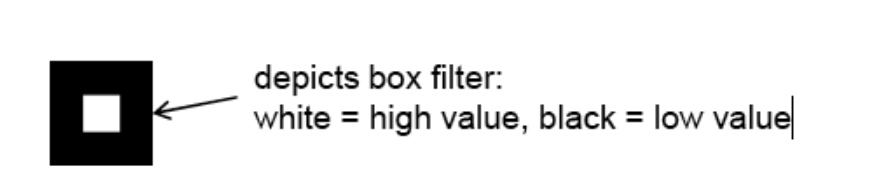
\includegraphics[width=0.6\textwidth]{figs/box_filter}
	\caption{Box Filter}\label{fig:box_filter}
\end{figure}
The box filter depicted in Figure \ref{fig:box_filter} is the exact same filter if we only keep the white part, i.e. the 1 entries. As the size of the box filter increases, the end result gets more and more blurry. 

\subsubsection{Isotropic Gaussian Filter}
\begin{figure}[H]
	\center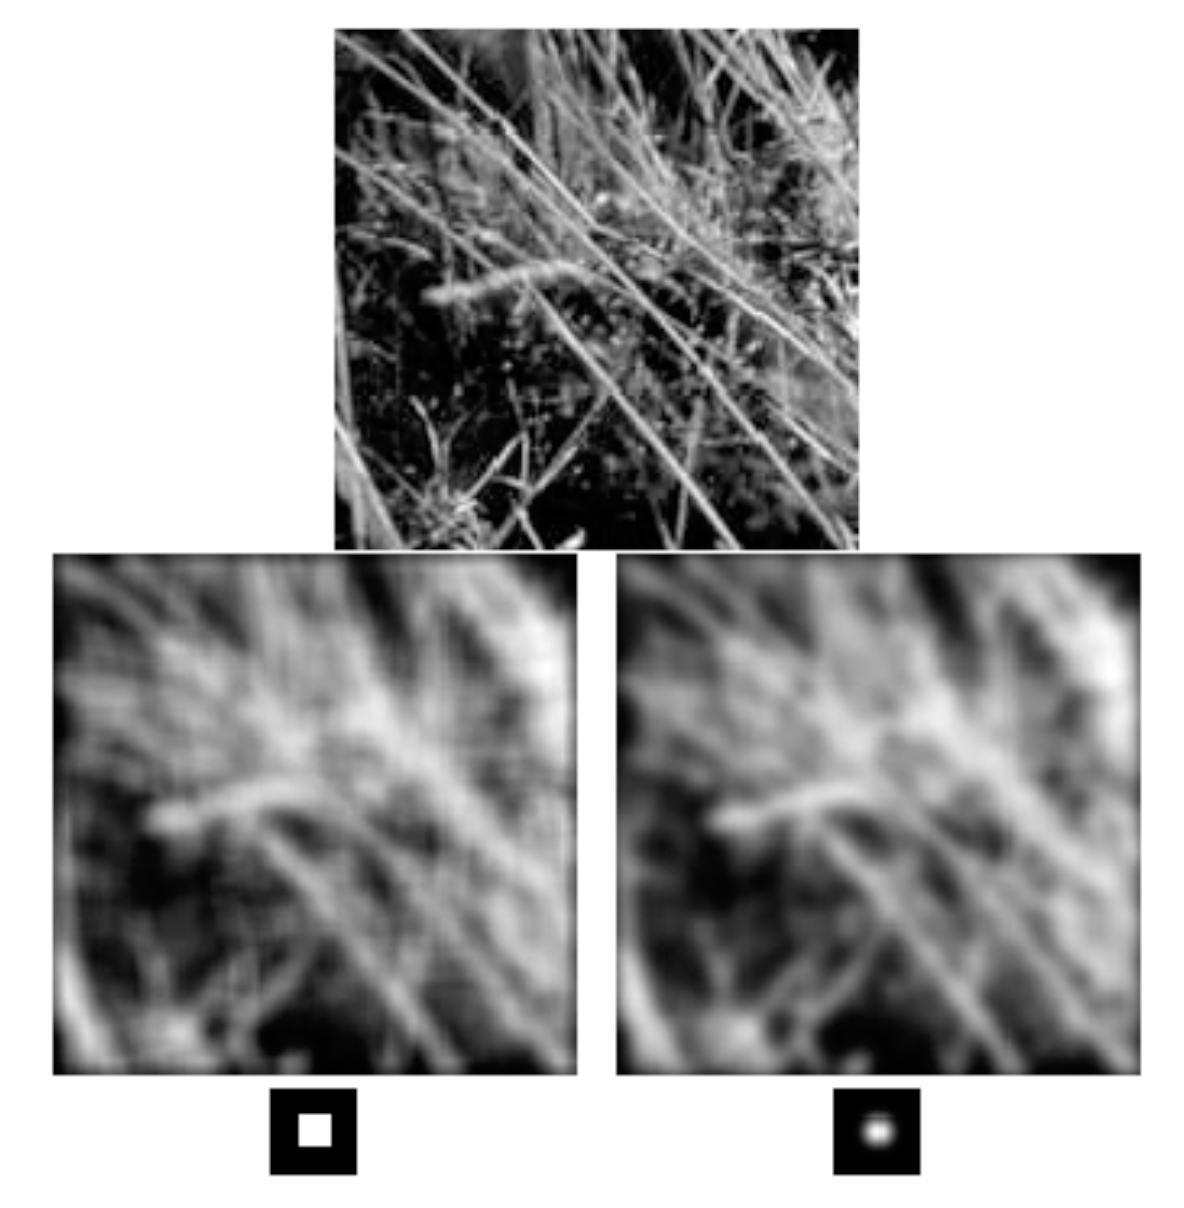
\includegraphics[width=0.6\textwidth]{figs/filter_comp}
	\caption{Comparison of filtered result using uniform filter (bottom left) and gaussian filter (bottom right)}
	\label{fig:filter_comp}
\end{figure}
Recall that the gaussian probability distribution is defined as 
\begin{equation}
	\text{Gaussian}(\bx; \boldsymbol{\mu}, \Sigma ) = (2 \pi)^{-\frac{k}{2}} \operatorname{det}(\Sigma)^{-\frac{1}{2}} e^{-\frac{1}{2}(\mathbf{x}-\boldsymbol{\mu})^{\top} \Sigma^{-1}(\mathbf{x}-\boldsymbol{\mu})}
\end{equation}
and we can mimic this to develop a filter that has entries mimicking values taken by the gaussian pdf. These filters produce results much nice than averaging in terms of smoothing, as we can see in Figure \ref{fig:filter_comp}.

\paragraph{Specification} The Gaussian Filter $G$ is parametrized by two parameters $\Sigma = \sigma I$ (isotropic) and $\boldsymbol{\mu}$. In application, $\boldsymbol{\mu}$ doesn't matter, we always want to make sure that the peak of the gaussian pdf corresponds to the centre pixel of the filter. The size of the filter depends on our choice of $\Sigma$, e.g. it doesn't make much sense if our kernel includes values more than $2\sigma$'s away. We also need to normalize all the taken values again, to make sure the filter we chose sums up to one!

\subsubsection{Non-isotropic Gaussian Filter}
In the most general case, Gaussian can be non-isotropic, meaning that its variance-covariance matrix \textit{\textbf{is not}} of form $\sigma I$ 

\subsection{Convolution}
The Convolution operation is defined as
\begin{equation}
	G(i, j)=\sum_{u=-k}^{k} \sum_{v=-k}^{k} F(u, v) \cdot I(i-u, j-v)
	\label{eq:conv}
\end{equation}
Notice that this is exactly the same as Correlation defined in Equation \ref{eq:generalfiltering} except that we are flipping the filter in both dimensions (bottom to top, right to left). \note{In the case of Gaussian / box filters, since the filter will be symmetric about both horizontal and vertical axis, $F \ast I = F \otimes I$.}

\subsubsection{Properties of Convolution}
Convolution is a Linear Operation, meaning that if $f, g$ and $h$ are three convolution operators, and $\lambda \in \real$ then
\begin{itemize}
	\item \textit{\textbf{Commutative}}: $f * g=g * f$
	\item \textit{\textbf{Associative}}: $f *(g * h)=(f * g) * h$
	\item \textit{\textbf{Distributive}}: $f *(g+h)=f * g+f * h$
	\item \textit{\textbf{Assoc. with scalar multiplier}}: $\lambda \cdot(f * g)=(\lambda \cdot f) * g$
\end{itemize}

\subsubsection{Convolution w/ Fourier Transforms}
The Fourier transform of two convolved images is the inner product of their individual Fourier Transforms, i.e.
\begin{equation}
	\mathcal{F}(f * g)= \langle \mathcal{F}(f), \mathcal{F}(g) \rangle
\end{equation}
\paragraph{Implications} The computational complexity of Fourier Transform is much lower than that of convolution. Also notice that inner products are fast to compute. \unsure{Confirm and finish this !}


\subsection{Separable Filters}
For a $K \times K$ sized filter / kernel, the process of performing a convolution requires $K^2$ operations per pixel, summing up to a total of $\#\text{pixels} \times K^2$ for an entire image. In many cases, though not all, we can speed this process up by (1) performing a 1-D horizontal convolution followed by (2) a 1D vertical convolution, requiring only $2K$ operations! When we can do this trick, we call the kernel ``separable''. And a filter is separable iff it is the outer product of two vectors (each a 1D filter):
\begin{equation}
	\exists?\, \bv, \bh \in \real^K, s.t.\,\, F=\mathbf{v} \mathbf{h}^{\top}	
\end{equation}

\subsubsection{Isotropic Gaussian as Separable Filters}
One famous example of separable filter that we are already familiar with is the Gaussian Filter, assuming isotropic variance. In such case the density breaks down into 
\begin{align}
	\text{Gaussian}(x, y; \boldsymbol \mu = \bzero, \Sigma = \sigma I) 
	&= \frac{1}{2 \pi \sigma^{2}} \exp \left\{-\frac{x^{2}+y^{2}}{\sigma^{2}}\right\} \\
	&= \left[\frac{1}{\sqrt{2 \pi} \sigma} \exp\left\{-\frac{x^{2}}{\sigma^{2}}\right\}\right] \cdot\left[\frac{1}{\sqrt{2 \pi} \sigma} \exp\left\{-\frac{y^{2}}{\sigma^{2}}\right\}\right]
\end{align}
Such factorization of gaussian pdf indicates us that we should have two 1-D filters that are 1-D gaussian each. 

\subsubsection{Moving Average as Separable Filters}
The na\"ive moving average filter that we encountered earlier is also separable, in which case
\begin{equation}
	F = \begin{bmatrix}
		1 & \hdots & 1 \\
		\vdots & \ddots & \vdots \\
		1 & \hdots & 1
	\end{bmatrix} / K^2 = \begin{bmatrix}
		1/K & \dots & 1/K
	\end{bmatrix}^\top  \begin{bmatrix}
		1/K & \dots & 1/K
	\end{bmatrix}
\end{equation}

\subsubsection{Edge Detector Kernel as Separable Filters}
The edge detector \unsure{Come back: left or right edge detector?}
\begin{equation}
	F = \begin{bmatrix}
		-1 & 0 & 1 \\
		-2 & 0 & 2 \\
		-1 & 0 & 1
	\end{bmatrix} / 8; \quad \bv = \begin{bmatrix}
		-1 & 0 & 1
	\end{bmatrix} / 2; \quad F = \bv^\top \bv
\end{equation}

\subsubsection{Separable-ness of Filters}
A systematic way of checking if a kernel is separable if by looking at the singular value decomposition of the filter. \textit{\textbf{If only one singular value is non-zero, the it is separable}}
\begin{equation}
	F=\mathbf{U} \Sigma \mathbf{V}^{\top}=\sum_{i} \sigma_{i} u_{i} v_{i}^{\top}
\end{equation}
with $\Sigma=\operatorname{diag}\left(\sigma_{i}\right)$. Then, we can get the vertical and horizontal filter through
\begin{equation}
	F_\text{vertical} \gets \sqrt{\sigma_{1}} \mathbf{u}_{1} \quad\quad F_\text{horizontal} \gets \sqrt{\sigma_{1}} \mathbf{v}_{1}^{\top }
\end{equation}
 

\section{Edge Detection}
\subsection{Characterization of Edges}
\subsubsection{Insights}
\begin{itemize}
	\item Edge detection involves mapping image to a set of \textit{\textbf{curves}} or \textit{\textbf{line segments}} or \textit{\textbf{contours}}.
	\item Such representation is more compact than pixels. Notice that for a coloured (ordinary, not HDR) $m \times n$ image, we will need $m \times n \times 3 \times 8$ bits to store all the information. However, for edges $m \times n$ would suffice. 
	\item They are particularly useful due to their invariance towards illumination - it thus helps computers see better. Aside: edges are also important for recognition for human. 
\end{itemize}

\subsubsection{Origin of Edges}
\begin{figure}[H]
\center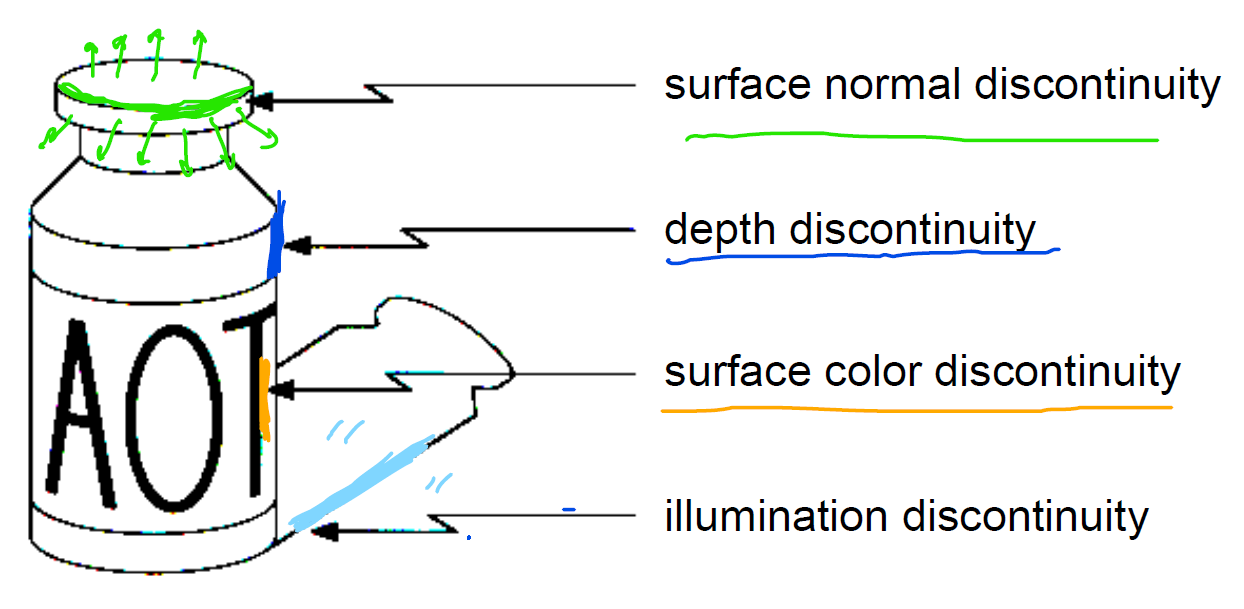
\includegraphics[width=0.6\textwidth]{figs/edge_types.png}
\caption{Four origins of edges \label{fig:edge_types}}
\end{figure}
Figure \ref{fig:edge_types} illustrates the four types of edges that can occur. 
\begin{itemize}
\item \textit{\textbf{Surface Normal Discontinuity}} is where surface normals change direction abruptly. 
\item \textit{\textbf{Depth Discontinuity}} is caused by depth discrepancy between two objects from the angle of the viewer. For example here in Figure \ref{fig:edge_types}, the background and the bottle causes a depth discontinuity. 
\item \textit{\textbf{Surface Colour Discontinuity}} is for example the edge of black text T on a white bottle. 
\item \textit{\textbf{Illumination Discontinuity}} is when there is a shadow causing difference in light. 
\end{itemize}

\subsubsection{Characterizing Edges}
\paragraph{Definition} An edge is a place of rapid change in image intensity function. The means that at places where edges occur, the intensity function should be steep, and the first derivative of the intensity at that position should correspond to extrema. 

\subsection{Convolution as Derivative - Measure of Rapid Change}
Consider an image $f(x, y)$ defined for $x\in \mathbb Z ^{\geq 1, \leq m}, y \in \mathbb Z ^{\geq 1 , \leq n}$, how can we differentiate this digital image given that it is not continuous? The answer is we take the first order forward discrete derivative (finite difference), i.e. 
\begin{equation}
\frac{\partial f(x, y)}{\partial x} \approx \frac{f[x+1, y] - f[x, y]}{1}
\end{equation}
and
\begin{equation}
\frac{\partial f(x, y)}{\partial y} \approx \frac{f[x, y + 1] - f[x, y]}{1}
\end{equation}

\paragraph{Correlation Filter}
Clearly we can implement the above as kernels, 
\begin{equation}
H_x = \begin{bmatrix}
	0 & 0 & 0 \\	
	0 & -1 & 1 \\
	0 & 0 & 0 \\
\end{bmatrix} \quad \text{and} \quad H_y = \begin{bmatrix}
	0 & 1 & 0 \\	
	0 & -1 & 0 \\
	0 & 0 & 0 \\
\end{bmatrix}
\end{equation}
then, we have
\begin{equation}
\left[ f \otimes H_x \right]_{(i, j)} = \left. \frac{\partial f(x, y)}{\partial x}\right|_{(i, j)} 
\quad \text{and} \quad 
\left[ f \otimes H_y \right]_{(i, j)} = \left. \frac{\partial f(x, y)}{\partial y}\right|_{(i, j)} 
\end{equation}

\subsubsection{Canonical Finite Difference Filters}
\paragraph{The Prewitt Kernel} is more symmetric, and averages each pixel from neighbouring pixels only. Also this filter applies a tiny blurring on the direction that it is not detecting edge. ($M_x$ is blurring for vertical direction. )
\begin{equation}
	M_x = 
	\begin{bmatrix}
		-1 & 0 & 1 \\
		-1 & 0 & 1 \\
		-1 & 0 & 1
	\end{bmatrix} \quad \text{and} \quad M_y = \begin{bmatrix}
		1 & 1 & 1 \\
		0 & 0 & 0 \\
		-1 & -1 & -1
	\end{bmatrix}
\end{equation}

\paragraph{Sobel Filter} is more common. Same as Prewitt, in the direction of that the kernel is not detecting edges, it applies a bit blurring effect. \textit{However, in Sobel, the blurring is a Gaussian blur.}  
\begin{equation}
	M_x = 
	\begin{bmatrix}
		-1 & 0 & 1 \\
		-2 & 0 & 2 \\
		-1 & 0 & 1
	\end{bmatrix} \quad \text{and} \quad M_y = \begin{bmatrix}
		1 & 2 & 1 \\
		0 & 0 & 0 \\
		-1 & -2 & -1
	\end{bmatrix}
\end{equation}

\paragraph{Roberts Kernel} detects diagonal edges; 
\begin{equation}
	M_x = \begin{bmatrix}
		0 & 1 \\
		-1 & 0
	\end{bmatrix} \quad \text{and} \quad M_y = \begin{bmatrix}
		1 & 0 \\
		0 & -1
	\end{bmatrix}
\end{equation}

\subsection{Image Gradient}
\subsubsection{Gradient Defined}
The gradient of an image $f: \real ^2 \rightarrow \real$ is defined, exactly the same as usual, as
\begin{equation}
	\nabla f=\left[\frac{\partial f}{\partial x}, \frac{\partial f}{\partial y}\right]
\end{equation}

\subsubsection{Edge Direction}
The gradient always points in the direction of most rapid change in intensity. This means that if
\begin{equation}
	\nabla f=\left[\frac{\partial f}{\partial x} \neq 0, \rightarrow 0\right]
\end{equation}
then that position corresponds to a vertical edge. If 
\begin{equation}
	\nabla f = \left[ \rightarrow 0, \frac{\partial f}{\partial y} \neq 0 \right]
\end{equation}
when we are at a horizontal edge. At a slanted edge, we will get
\begin{equation}
	\nabla f=\left[\frac{\partial f}{\partial x} \neq 0 , \frac{\partial f}{\partial y} \neq 0 \right]
\end{equation}

\subsubsection{Gradient Direction}
The gradient direction (i.e. orientation of edge normal) is given by
\begin{equation}
	\tan  \theta = \frac{\partial f}{\partial y} / \frac{\partial f}{\partial x} \implies \theta = \arctan \left(\frac{\partial f}{\partial y} / \frac{\partial f}{\partial x}\right)
\end{equation}

\subsubsection{Edge Strength}
The edge strength is given by the $L_2$ norm of the gradient vector:  
\begin{equation}
	\|\nabla f\|=\sqrt{\left(\frac{\partial f}{\partial x}\right)^{2}+\left(\frac{\partial f}{\partial y}\right)^{2}} 
\end{equation}

\subsection{Effects of Noise}
\begin{figure}[H]
	\center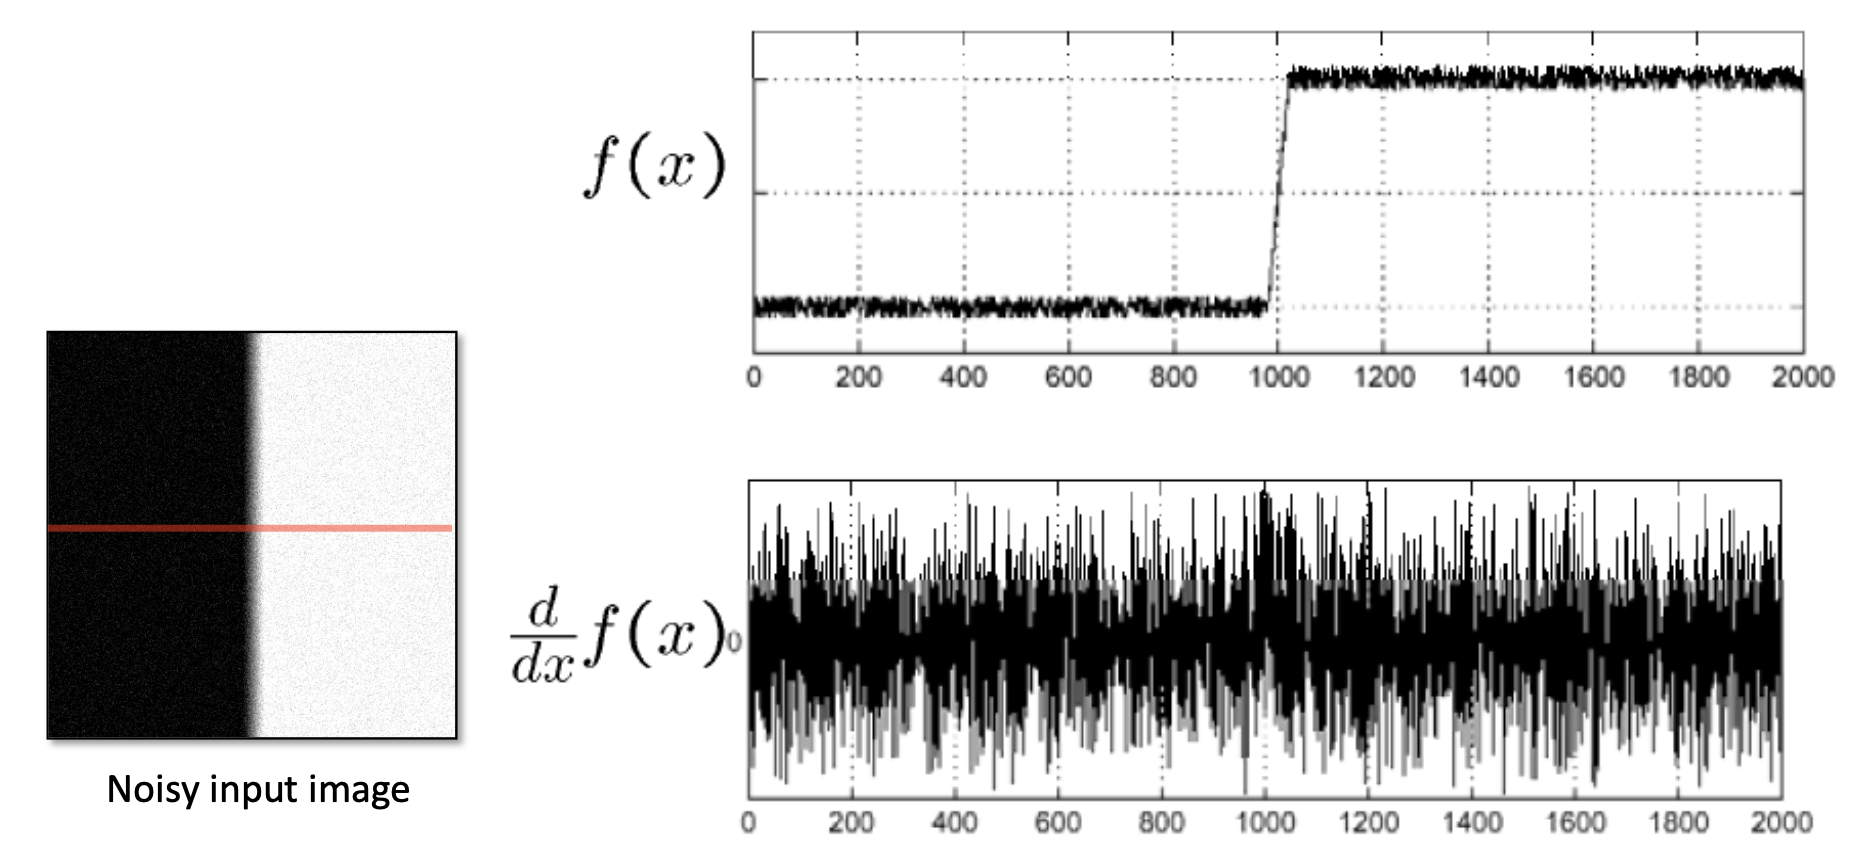
\includegraphics[width=0.6\textwidth]{figs/noisy_input}
	\caption{\label{fig:noisy_input}Illustration of noisy input problem.}
\end{figure}
As shown in Figure \ref{fig:noisy_input}, when we have edges that are not sharp, the image is noisy and thus cause the derivative messy. 

\subsubsection{Overcoming Noisiness \label{sec:overcome_noisiness}}
The solution to the problem is easy. We simply first smooth the input signal and then look for edges. I.e., for an input image $f$, and noise reduction filter (e.g. Gaussian) $h$, we find extremum in $\frac{\partial }{\partial x}\left( h \ast f \right)$

\subsubsection{Faster Method Through Conv / Corre}
We know that correlation is associative, i.e. $f *(g * h)=(f * g) * h$. We can use this property to speed up our method of overcoming noisiness mentioned in Section \ref{sec:overcome_noisiness}. Consider an image $I\in \mat{m}{n}$, smoothing filter $G\in \mat{k}{k}$, and $x$-derivative kernel $F \in \mat{k}{k}$. Then, 
\begin{align}
	\frac{\partial }{\partial x} (G \ast I) 
	&= F \ast ( G \ast I )) \\
	&= (F \ast G) \ast I\label{eq:fast_filter_conv}
\end{align}
and since $k \ll m, n$, Equation \ref{eq:fast_filter_conv} i  s much faster to compute. 

\subsubsection{Generalization: Derivative Theorem of Convolution}
For a image $f$, with filter $h$, we have
\begin{equation}
	\frac{\partial}{\partial x}(h * f)=\left(\frac{\partial h}{\partial x}\right) * f=h *\left(\frac{\partial f}{\partial x}\right)
\end{equation}
i.e. rather than convolving the image with the filter and then take the derivative, we first get the derivative of the filter and convolve the result with the image. \note{This saves us one operation.}

\subsubsection{Remark: on Gaussian Derivative Filters' Parameter}
We know that if we apply the derivative of gaussian as a filter to an image, it finds the edges on the smoothened version of the image. However, the detected structures differ depending on the Gaussian's std. deviation chosen. 
\begin{itemize}
	\item If we have a large $\sigma$, then the filter detects edges of larger scale
	\item else if we have a small $\sigma$, we will be detecting finer structures. 
\end{itemize}

\subsection{Canny's Edge Detector}
\subsubsection{Procedure}
\begin{enumerate}
	\item Filter images with derivative of gaussian (horizontal and vertical directions)
	\item Find magnitude and orientation of gradient
	\item Non-maximum suppression
	\item Linking and thresholding (hysteresis)
	\begin{itemize}
		\item Define two thresholds: low and high
		\item Use the high threshold to start edge curves and the low threshold to continue them
	\end{itemize}
\end{enumerate}

\paragraph{Parameters}
There are three parameters (hyper-parameters) that we need to fix for the algorithm, namely scale of Gaussian in step 1, and low / high thresholds in step 4. There are no magical way in tuning them, so it requires quite a lot of experimentation. 

\subsubsection{Non-Maximum Suppression (Thick Edges Problem)}
\begin{itemize}
	\item check if pixel is local maximum along gradient direction?
	\item if yes, take it; otherwise neglect it. 
\end{itemize}
i.e. in an image $f$ we take $(i, j)$ if in a local area 
\begin{equation}
	\forall (i', j'), I(i, j) > I (i',j')
\end{equation}
then keep $\norm{\nabla f} \gets \norm{\nabla f}$ otherwise $\norm{\nabla f} \gets 0$

\subsubsection{Hysteresis Thresholding (Discontinuous Edges Problem)}
\begin{itemize}
	\item Filter at high threshold, getting strong edges. Call this result $S$
	\item Filter at low threshold, getting weak edges, call this result $W$
	\item Along directions where edges develop in $S$, if there is an edge in $W$ at the same spot, then we adopt it. Continue until a point where norm of gradient is below the low threshold. 
\end{itemize}


\subsection{Laplacian of Gaussians: Another Approach to Edge Detection}
Consider (noisy) image $f$, and a Gaussian filter $h$. We have the laplacian of $h$, as $\frac{\partial^{2}}{\partial x^{2}} h$, and then we calculate 
\begin{equation}
	\left(\frac{\partial^{2}}{\partial x^{2}} h\right) \ast f
\end{equation}
where zero-crossings in the resulting graph correspond to edges. 

\subsection{Auxiliaries} 
\subsubsection{Connection: Sobel Filter and Gaussian Blur} 
We already know that 
\begin{equation}
	F *(G * I)=(F * G) * I
\end{equation}
and suppose 
\begin{equation}
	F = \begin{bmatrix}
		-1 & 0 & 1
	\end{bmatrix}\quad \text{and} \quad \begin{bmatrix}
		1 & 2 & 1 \\
		2 & 4 & 2 \\
		1 & 2 & 1 
	\end{bmatrix} / 14
\end{equation}
then if we use the convolution sequence on the right, we will get 
\begin{equation}
	\left[
		\begin{array}{ccccc}
			-1 & -2 & 0 & 2 & 1 \\
			-2 & -4 & 0 & 4 & 2 \\
			-1 & -2 & 0 & 2 & 1
		\end{array}
	\right] \in \mat{3}{5}
\end{equation}
as an intermediate result. But this non-square result is not ``nice''. So more commonly we use 
\begin{equation}
	G = 
	\begin{bmatrix}
		1 & 2 & 1 
	\end{bmatrix}^ \top / 4
\end{equation}
in which case 
\begin{equation}
	F * G = \begin{bmatrix}
		-1 & 0 & 1 \\
		-2 & 0 & 2 \\
		-1 & 0 & 1
	\end{bmatrix}
\end{equation}
and we notice that the result is exact the same as Sobel Filter we mentioned earlier. 

\section{Image Pyramids}
In Linear Filter section, we talked about the technique of using correlation / convolution to aid us find Waldo in a picture. However, that method relies on the filter and the matching portion in the image being the same size. What should we do when we have the template, but just a thumbnail image of the filter? 

\subsection{Image Sub-Sampling}
The goal is very simple, how do we make a smaller sized image out of an original image? e.g. 1/4 sized, 1/8 sized...
\subsubsection{Na\"ive Solution} Simply remove some columns and rows based on a predetermined rule, e.g. remove one in every two row / column. In our example, the remaining pixel makes a 1/2 sized image. We can do this again and again, creating an $1 / 2^n$ sized image. 
\paragraph{Pitfall - Natural Image} This very simple solution creates images that look very crufty (containing very sharp noises). 
\paragraph{Pitfall - Synthetic Image} In a computer synthesized image where there is a box, with line width of 1px. Now I wish to resize the image by a factor of 2 by taking away every other column and every other row (1st, 3rd, 5th, etc). But then, if any of the column / row of pixel in the image is the same as the ``every other row'' discarded, then we have problem - our box will have missing sides. And this is not a rare event. 

\subsubsection{Aliasing}
Aliasing could occur when we sample from a source signal, and due to limitations in the sampling rate / density we get a completely different sampled signal output. We say that the sampling rate is not high enough to capture the amount of detail in the original signal. \info{This is commonly seen when we take a photograph for a digital screen and view it on a display with not high-enough resolution. } 

\subsubsection{Nyquist Rate (Nyquist-Shannon Theorem)}
Poor sampling creates aliasing. To do sampling right, we need to understand the structure of the input signal. The minimum sampling rate is called the Nyquist Rate\footnote{nameed after Sir Harry Nyquist. \url{https://en.wikipedia.org/wiki/Nyquist\%E2\%80\%93Shannon_sampling_theorem}}. Harry states that 
\begin{itemize}
	\item One should look at the frequencies of the signal, and
	\item find the highest frequency via Fourier Transform. 
	\item To sample properly, you need to sample with at least twice that highest frequency. 
\end{itemize}
In short, we need
\begin{equation}
	\text{Sampling Freq.} > 2 \times \text{Max Freq. Component of Original Signal}
\end{equation}

\subsubsection{Gaussian Pre-Filtering}
We now see that high frequency signals are ``some-what'' the problem in signal sub sampling. In image, this typically correspond to sharp edges. The solution to this problem is to use a Gaussian Filter to help us do a pre-filtering. The blurring helps aggregate, at each resulting pixel positions, information from pixels around, making the image smoother \footnote{I think this can also be explained by Statistical Multiplexing.} 

\paragraph{Theory Behind}
Recall that Gaussians are exponential, so we can write the pdf $f(x)$ up to a scaler multiplicand difference 
\begin{equation}
	f(x) = \exp\{-ax^2\} \propto \frac{1}{\sigma \sqrt {2 \pi }} \exp\left\{\frac{-x^2}{2\sigma^2} \right\}
\end{equation}
where $a = 1 / 2\sigma^2$. Then, the Fourier Transformation is
\begin{align}
	F(f(x)) 
	&= \int_{-\infty}^{+\infty} e^{-a x^{2}} e^{-2 \pi i k x} \mathrm d \, x = f(f(x)) (k) \\
	&= \int_{-\infty}^{+\infty} e^{-ax^2} \left( \cos ( -2\pi i k x ) + i\sin ( -2\pi i kx )\right) \mathrm d \, x \\
	&= \int_{-\infty}^{+\infty} e^{-ax^2} \cos ( -2\pi i k x ) \mathrm d \, x \\
	&= \sqrt{\frac{\pi}{a}} \exp \left\{ \frac{-\pi^2 k^2}{a} \right\} 
\end{align}

\subsubsection{Image Pyramids}
A sequence of images created with Gaussian blurring and downsampling is called a Gaussian Pyramid. \info{In CV, this is called a \textit{mip map}}We represent a $N \times N$ sized image as a pyramid of $1 \times 1$, $2 \times 2$, ..., $2^k \times 2^k$ images, assuming $N = 2^k$. 

\subsection{Image Up Sampling}
Now we consider the opposite question: if an image is too small, how can we make it 10 times larger? 

\subsubsection{Na\"ive Solution}
We can repeat each row and column 10 times and create a ``quasi'' sized up image. 
\paragraph{Pitfall} We notice that this method of sizing up just made the size of the image larger, but it does so by creating blobs of pixels representing the same pixel. This result is not desirable. 

\subsubsection{1-D Signal Linear Interpolation}
We can make a linear interpolation between neighbouring discrete points in the input signal to create a better up sampling solution. Suppose input is $F(x)$, and between points $x_1$ and $x_2$, we wish to sample a $x$. Then, 
\begin{equation}
	x = \alpha x_1 + (1 - \alpha ) x_2, \alpha \in (0, 1)
\end{equation}
and the estimated signal strength (by linear interpolation) is
\begin{equation}
	\hat F(x) = \alpha F(x_1) + ( 1 - \alpha ) F (x_2) , \alpha \in (0, 1)
\end{equation}
Rewriting and substituting gives us the final formula of 
\begin{equation}
	\hat F(x) = \frac{x_{2}-x}{x_{2}-x_{1}} F\left(x_{1}\right)+\frac{x-x_{1}}{x_{2}-x_{1}} F\left(x_{2}\right)
\end{equation}

\subsubsection{1-D Linear Interpolation Via Convolution}
Consider 1-D input signal $F$, and we first ``expand'' it (filling gaps between signal points with 0s). We call this expanded version $G'$. Then, to get final result $G$, it suffices to compute
\begin{equation}
	G = h \ast G'
\end{equation}

\begin{figure}[H]
	\center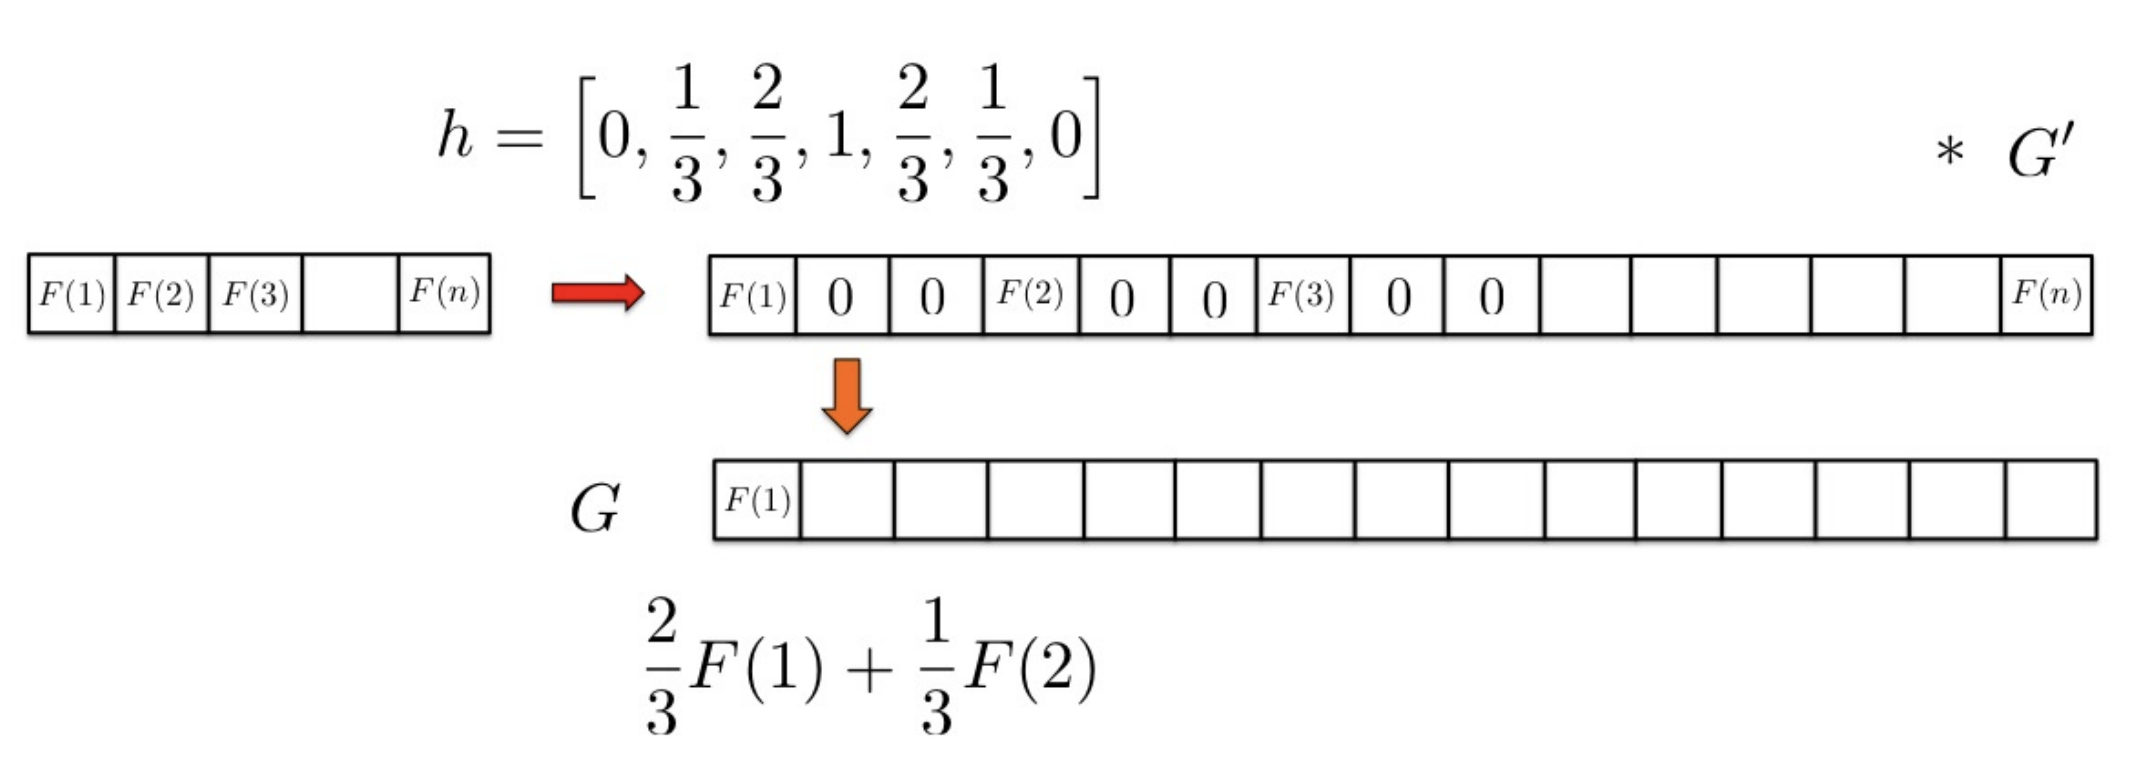
\includegraphics[width=0.7\textwidth]{figs/up_sample_conv}
	\caption{Worked example of up sampling with linear interpolation via convolution. $h$ shown is the convolution filter, $G'$ is the expanded input, and $G$ is final result. \label{fig:up_sample_conv}}
\end{figure}

\paragraph{Example ($d = 3$)} We can work out a $h$ in a simple case of $d = 3$, as shown in Figure \ref{fig:up_sample_conv}. But what about the general case? What should be my reconstruction filter $h$, such that $G = h \ast G'$?

\paragraph{General Case} In general, we can find $h$ using
\begin{equation}
	h=\left[0, \frac{1}{d}, \ldots, \frac{d-1}{d}, 1, \frac{d-1}{d}, \ldots, \frac{1}{d}, 0\right]
\end{equation}
where $d$ is the up-sampling factor to help determine the reconstruction filter. Notice that the filter is symmetric. 


\subsubsection{1-D Non-Linear Interpolations}
Previously we saw that we can use linear interpolation between points to help us reconstruct signals in up sampling. We can also use nonlinear functions as interpolation, for example
\begin{itemize}
	\item \begin{equation}
		\operatorname{sinc}(x) \equiv \left\{\begin{array}{ll}
			1 & \text { for } x=0 \\
			\frac{\sin x}{x} & \text { otherwise }
		\end{array}\right.
	\end{equation} produces so called ``ideal'' reconstruction
	\item $\prod(x)$ produces nearest neighbour interpolation. 
	\item $\Lambda(x)$ is our familiar linear interpolation
	\item $\text{Gauss}(x)$ makes gaussian reconstruction
\end{itemize}


\subsubsection{2-D Image Interpolation}


\section{Interest (Key) Point Detection}
\subsection{Review: Taylor Expansion}
In general, if we have a function $f$ that is $\mathcal C^1$\footnote{Will need $\mathcal C^\infty$ if we want entire taylor series, but we are just using first order approximation here. } around a point $a$, than for all $x$ in a neighbour hood of $a$, 
\begin{equation}
	f(x) \approx f(a) + f'(a)(x - a)
\end{equation}
Let's call $x - a$ as $y$, and since the value is small, lets call $a$ as $\Delta y$. Then,
\begin{equation}
	f(y + \Delta y) = f(y) + f'(y)\Delta y
\end{equation}
This also works for $\real^2 \rightarrow \real$ functions, and in particular works for images, in which
\begin{equation}
	I(x+u,y+v) \approx I(x, y) + u\partial_x I(x, y) + v\partial_y I (x, y)
\end{equation}

\subsection{The Problem and Goal}
Given two (or more) images of the same subject or very similar subjects, identify (at least some points in both images).
\begin{itemize}
	\item We have to be able to run the detection procedure independently per image,
	\item we need to generate enough points to increase our chance of detecting matching pts, 
	\item we should not generate too many key pts, or otherwise the algorithm will be really slow in checking matching pairs. 
\end{itemize}
 
\subsubsection{Na\"ive Point Choosing Criteria}
We want to detect points that represent ``corners'' of objects in the image. This makes these patches more unique. If all the edges of corners are $x$ and $y$ axis aligned, then we can just choose points where both $x$ and $y$ directional partial derivatives are large. But this clearly is not a general solution. 

\subsection{Harris Corner Detector}
\subsubsection{Second Moment Matrix / Structure Tensor}
Define the weighted sum (called weighted sum of squares difference)
\begin{equation}
	E(u, v) = \sum_x \sum_y w(x, y)\left( I(x, y) - I(x + u, y + v) \right)^2
\end{equation}
Here $w(\cdot, \cdot)$ is called a window or weight function, $I(\cdot, \cdot)$ is called the intensity function. Our final goal is to make $E(u, v)$ large for any small $(u, v)$. We can expand $E$,
\begin{align}
	E_{wssd}(u, v) 
	&= \sum_x\sum_y w(x, y) \left( I(x, y) - I(x + u, y + v) \right)^2 \\
	&\approx \sum_x\sum_y w(x, y) \left( I(x, y) - I(x, y) - u\partial x I(x, y) - v\partial_y I(x,y) \right)^2 \\
	&= \sum_x \sum_y w(x, y) (u^2 \partial_x I \partial x I + 2uv \partial_xI \partial_yI + v^2 \partial_y I \partial_y I) \\
	&= \sum_x \sum_y w(x, y) \begin{bmatrix}
		u & v
	\end{bmatrix}\begin{bmatrix}
		(\partial_x I )^2 & \partial_x I \partial_y I \\
		\partial_x I \partial_y I & (\partial_y I )^2 
	\end{bmatrix}\begin{bmatrix}
		u \\ v 
	\end{bmatrix}
\end{align}
since the $u, v$ extraneous variables, we can move them out, 
\begin{align}
	E_{wssd}(u, v) = \begin{bmatrix}
		u & v
	\end{bmatrix} \underbrace{\left( \sum_x \sum_y w(x, y)\begin{bmatrix}
		(\partial_x I )^2 & \partial_x I \partial_y I \\
		\partial_x I \partial_y I & (\partial_y I )^2 
	\end{bmatrix}\right)}_{M\in\mat{2}{2}}  \begin{bmatrix}
		u \\ v 
	\end{bmatrix}
\end{align} 

\subsubsection{Properties of Structure Tensor}
For convinience, let $\dagger = \begin{bmatrix}
		(\partial_x I )^2 & \partial_x I \partial_y I \\
		\partial_x I \partial_y I & (\partial_y I )^2 
	\end{bmatrix}$
\begin{itemize}
	\item Clearly $W$ is symmetric and real, so it must have all real eigenvalues. 
	\item $\det \dagger = 0$, so at least one of the eigenvalues of $\dagger$ is zero: $\lambda_1 = 0$ and $\lambda_2 \geq 0$. We say that $\dagger$ is a \textit{\textbf{positive semi-definite matrix}}.
	\item $\det M = \sum_x\sum_y w(x, y) \det (\dagger )$. The sum of positive semi-definite matrices is also positive semi-definite. Hence the eigenvalues of $M$ are all $\geq 0$. (there are two of them).
	\item Since it is symmetric and real, according to Spectral Theorem, this matrix is diagonalizable, and the rotation matrices are orthonormal.\footnote{Orthonormal: $V^\top V = VV^\top = I$ and $V^\top = V^{-1}$}We have 
	\begin{equation}
		M  = V \begin{bmatrix}
			\lambda_1 & 0 \\
			0 & \lambda_2
		\end{bmatrix} V^{-1} = V \begin{bmatrix}
			\lambda_1 & 0 \\
			0 & \lambda_2
		\end{bmatrix} V^{\top}
	\end{equation} 
\end{itemize}

\subsubsection{Weight Sum of Squared Difference Maximization}
We saw above that we can diagonalize $M$, and if we expand this into $E_{wssd}$, then 
\begin{equation}
	E_{wssd}(u, v) = \begin{bmatrix}
		u & v
	\end{bmatrix} V \begin{bmatrix}
		\lambda_1 & 0 \\
		0 & \lambda_2
	\end{bmatrix} V^{-1} \begin{bmatrix}
		u \\ v
	\end{bmatrix}
\end{equation}
and this is big when both the two eigenvalues $\lambda_1$ and $\lambda_2$ are large. 

\subsubsection{Reverse Construction of Corners from WSSD Max Vals. }
Above we saw the relationship between $E_{wssd}$ and the eigenvalues, now we use this relationship to find out where in the image are the corners. 
\begin{itemize}
	\item If both $\lambda$'s are small: Boring areas, not much change
	\item else if both $\lambda$'s are big: corner!
	\item else if just one of them is big, then it is an edge. 
\end{itemize}

\subsubsection{Harris Corner Detector (Harris and Stephens, 88')} \info{This is a heuristic function that is high when both eigenvalues are large, and low when at least one eigenvalue os small. }
\begin{equation}
	R = \lambda_{0} \lambda_{1}-\alpha\left(\lambda_{0}+\lambda_{1}\right)^{2}=\operatorname{det}(M)-\alpha \cdot \operatorname{trace}(M)^{2}
\end{equation}
where $R$ is rotationally invariant and downweighs edge-like features where $\lambda_1 \gg \lambda_0$. $\alpha$ here is a hyper-parameter that is typically $0.04$ to $0.06$. If we plot R on axis of $\lambda_1$ and $\lambda_2$, then we will see 
\begin{itemize}
	\item when $\lambda_1$ and $\lambda_2$ both large, then $R$ will be large
	\item when they are both small, $R$ will be close to zero
	\item and when one of them small, the other large, $R$ will be negative. 
\end{itemize}

\paragraph{Note on Interchanging Notation} Notice that 
\begin{equation}
	\det M = \det V \det \begin{bmatrix}
		\lambda_1 & 0 \\
		0 & \lambda_2
	\end{bmatrix} \det V^{-1} 
\end{equation}
but since $V$ is orthonormal, and importantly a rotation matrix, it has a determinant of $1$. \footnote{Recall that determinant can be defined as the change of volume of unit square / cube after transformation. Rotating doesn't change the volume of the shape, so determinant is 1. } Hence, $\det M = \lambda_1\lambda_2$. 

\paragraph{Using Non-explicit Values} We can notice that the formula is in terms of det and trace operators, rather than just of the eigenvalues. Although these two forms are same mathematically, they have different compute time. (you don not need to compute eigenvalues!)

\subsubsection{Shi and Tomas, 94'}
Shi and Tomas, 94' proposed using the smallest eigenvalue of $M$, i.e. $\lambda_0^{-1/2}$

\subsubsection{Trigges, 04'}
Suggested 
\begin{equation}
	\lambda_0 - \alpha \lambda_1
\end{equation}
also reduces the response at 1D edges, where aliasing errors sometimes inflate the smaller eigenvalue. 

\subsubsection{Brown et al, 05'}
Suggested using the harmonic mean
\begin{equation}
	\frac{\operatorname{det}(M)}{\operatorname{trace}(M)}=\frac{\lambda_{0} \lambda_{1}}{\lambda_{0}+\lambda_{1}}
\end{equation}

\section{Motion and Optical Flow}
Perceiving, understanding and predicting motion is an important. Obviously, in this case the minimum amount of frame that we will need is two. Even the intelligent human brain can be fooled - we have all seen those static picture that seems to be moving. The question we wish explore in this section are
\begin{itemize}
	\item Extract visual features\footnote{E.g. Edges, corners, textures, objects are all so called visual features} (corners, textured areas) and ``track'' them over multiple frames
	\item Recover image motion at each pixel from spatiotemporal image brightness variations. This is called \textit{\textbf{Optical Flow}}.
\end{itemize}
 
\paragraph{Applications}
\begin{itemize}
	\item We may wish to achieve video stabilization (removing shaking), 
	\item analyzing moving objects in a (series of?) static frame
\end{itemize}

\paragraph{Feature Tracking}
Given two subsequent frames, say we want to estimate the point translation. Some assumptions that we make are (as proposed in the original Optical Flow paper; these assumptions are very strong)
\begin{itemize}
	\item Brightness constancy: projection of the same point looks the same in every frame, 
	\item small motion: points fo not move very far,
	\item spatial coherence: points (in a patch) move like their neighbours
\end{itemize}

\subsection{Brightness Constancy Constraint}
Suppose we have video and at time $t$, pixel location $(x, y)$ have brightness level $I(x, y, t)$. Then, if during time $t \rightarrow t + 1$ it had a displacement $(u, v)$, then it must be that
\begin{equation}
	I(x, y, t)=I(x+u, y+v, t+1)
\end{equation}
We can expand RHS, using Taylor approximation, around $(x, y, t)$, 
\begin{equation}
	I(x+u, y+v, t+1) \approx I (x, y, t) + u \partial_x I + v\partial_y I + 1 \partial_t I
\end{equation}
then we can reorder
\begin{equation}
	I(x+u, y+v, t+1) - I(x, y, t) = \approx u \partial_x I + v\partial_y I + 1 \partial_t I\label{eq:brightness constancy equation taylor expanded}
\end{equation}
But since we assumed brightness constancy, the LHS of Equation \ref{eq:brightness constancy equation taylor expanded} must be at least very close to zero. Then,
\begin{align}
	& u \partial_x I + v\partial_y I + 1 \partial_t I = 0 \\
	\implies & \nabla I \cdot \begin{bmatrix}
		u & v
	\end{bmatrix} ^\top + \partial_t I = 0  \label{eq:brightness constraint equation}
\end{align}
where $\nabla I$ is obtained by treating $t$ as extraneous. We notice that our goal is to solve the image motion vector $\begin{bmatrix}
	u & v
\end{bmatrix}^\top$, but we have only one equation for two unknown variables. 

\subsubsection{Pitfall} The component of the motion perpendicular to the gradient (parallel to edge) cannot be measured. If $(u, v)$ satisfies the brightness constraint equation (Equation \ref{eq:brightness constraint equation}), then so does $\left(u+u^{\prime}, v+v^{\prime}\right)$ if $\nabla I \cdot\left[\begin{array}{ll}
u^{\prime} & 
v^{\prime}
\end{array}\right]^\top =0$.\footnote{Since $\nabla I \cdot \begin{bmatrix}
	u + u' & v + v'
\end{bmatrix}^\top = \nabla I \cdot \begin{bmatrix}
	u  & v 
\end{bmatrix}^\top + \nabla I \cdot \begin{bmatrix}
	u' & v'
\end{bmatrix}^\top$ but $\nabla I \cdot \begin{bmatrix}
	u' & v'
\end{bmatrix}^\top$ could be potentially zero if the motion $\begin{bmatrix}
	u' & v'
\end{bmatrix}$ is along direction perpendicular to gradient. }This tells us that the brightness Constancy Constraint will not help us recover motion along direction perpendicular to image gradient. 

\subsection{Ambiguities}
\subsubsection{The Aperture Problem}
The aperture which was used to capture a motion can limit the way we interpret the motion. See a gif from wikipedia: \url{https://en.wikipedia.org/wiki/Motion_perception#The_aperture_problem} which illustrates this phenomenon. In na\"ive words, we cannot recover motion that was not seen. 

\subsubsection{The Barber Pole Illusion}
The revolving pole at entrance to barbers is really just revolving, but we perceive it as if it was moving upwards. 

\subsection{Spatial Coherent Constraint: Solving Ambiguities}
The solution lies within how we can get more equations for a pixel. We need help from the Spatial Coherent Constraint. Assume that a pixel's neighbours have the same motion vector $(u, v)$, and if we assume a $5\times 5$ window, that gives us $25$ equations per pixel, then we will have
\begin{equation}
	\forall \,\,\text{pixel $\bp$ in the 5 by 5 window}, \nabla I (\bp) \cdot \begin{bmatrix}
		u & v
	\end{bmatrix}^\top + \partial_t I (\bp) = 0
\end{equation}
Now we can expand the for all quantifier into a matrix operation, 
\begin{equation}
	\begin{bmatrix}
		\partial_x I (\bp_1) & \partial_y I (\bp_1) \\
		\vdots & \vdots \\
		\partial_x I (\bp_{25}) & \partial_y I (\bp_{25})
	\end{bmatrix} \begin{bmatrix}
		u \\ v
	\end{bmatrix} + \begin{bmatrix}
		\partial_t I (\bp_1) \\
		\vdots \\
		\partial_t I (\bp_{25})
	\end{bmatrix} = 0 
\end{equation}
and we rearrange it into a standard linear system form ($A \bd = \bb$),\footnote{$A\in \mat{25}{2}, \bd \in \mat{2}{1}, \bb \in \mat{25}{1}$. Here $\bd$ is the motion vector that is unknown and we want to solve for it. }
\begin{equation}
	\underbrace{\begin{bmatrix}
		\partial_x I (\bp_1) & \partial_y I (\bp_1) \\
		\vdots & \vdots \\
		\partial_x I (\bp_{25}) & \partial_y I (\bp_{25})
	\end{bmatrix}}_{\triangleq A} \underbrace{\begin{bmatrix}
		u \\ v
	\end{bmatrix}} _{\triangleq \bd} = \underbrace{- \begin{bmatrix}
		\partial_t I (\bp_1) \\
		\vdots \\
		\partial_t I (\bp_{25})
	\end{bmatrix}}_{\triangleq \bb}
\end{equation}
\subsubsection{Lucas-Kanade Equation: Least Squares Solution} Least Squares Solution for the motion vector $\bd$ is given by
\begin{multline}
	A^\top A \bd = A^\top\bb \quad\iff \\ \quad \left[\begin{array}{cc}
		\sum_{\bp '} \partial_x I(\bp) \partial_x I(\bp) & \sum_{\bp '} \partial_x I(\bp) \partial_y I(\bp) \\
		\sum_{\bp '} \partial_x I(\bp) \partial_y I(\bp) & \sum_{\bp '} \partial_y I(\bp) \partial_y I(\bp)
		\end{array}\right]\left[\begin{array}{l}
		u \\
		v
		\end{array}\right] =-\left[\begin{array}{c}
		\sum_{\bp '} \partial_x I(\bp) \partial_t I(\bp) \\
		\sum_{\bp '} \partial_y I(\bp) \partial_t I(\bp)
	\end{array}\right]\label{eq:lucas kanade equation}
\end{multline}
where the summations are over all pixels in the $K \times K$ window. (In our case, $5\times 5$). Equation \ref{eq:lucas kanade equation} is called the Lucas-Kanade Equation. 
\subsubsection{Connection: Second Moment Matrix}
We can notice that 
\begin{equation}
	A^\top A = \left[
		\begin{array}{cc}
			\sum_{\bp '} \partial_x I(\bp) \partial_x I(\bp) & \sum_{\bp '} \partial_x 	I(\bp) 	\partial_y I(\bp) \\
			\sum_{\bp '} \partial_x I(\bp) \partial_y I(\bp) & \sum_{\bp '} \partial_y I(\bp) 	\partial_y I(\bp)
		\end{array}
	\right]
\end{equation}
is precisely the second moment matrix. 

\subsubsection{Solvability Condition}
Optimal motion vector satisfies Lucas-Kanade Equation (Equation \ref{eq:lucas kanade equation}). It takes the form $A^\top A \bd = A^\top \bb$ and then ideally, we can solve $\bd = (A^\top A)^{-1} (A^\top \bb)$. Clearly it is not always ideal, so we summarize the solvability conditions as follows:
\begin{itemize}
	\item $A^\top A$ is invertible, i.e $\det (A^\top A) \neq 0$
	\item $A^\top A$ should not be too small due to noise: eigenvalues $\lambda_1, \lambda_2$ of $A^\top A$ should not be too small\footnote{RWe need this to be not close to singular, if it is close to singular, it's determinant will be close to zero, and the inverse will blowup. }
	\item $A^\top A$ should be well conditioned: $\max \{\lambda_1, \lambda_2\} / \min \{\lambda_1, \lambda_2 \}$ should not be too large. 
\end{itemize}

\paragraph{Importance of Eigenvectors} The eigenvectors here summarizes the distribution of gradient of the image $I$, within this window of $K \times K $. 
\begin{itemize}
	\item Suppose that the two eigenvectors are such that $\lambda_1 \geq \lambda_2$, and they have respective eigenvectors $\be_1$ and $\be_2$. Then we know that $\be_1$ is the direction that is maximally aligned with the gradient of the image in the $K \times K$ window. Let's now further suppose that $\lambda_1 > 0 \wedge \lambda_2 = 0$, then the gradient is always a multiple of $\be_1$, since there is no eigen-compinent from $\be_2$ due to $\lambda_2 = 0$. This is the case if and only if $I$ varies along with the direction $\be_1$ and is constant along $\be_2$. Edges!
	\item If $\lambda_1 = \lambda_2$, then the gradient in the $K \times K$ window has no prominent direction, which happens when we have rotational symmetry within the window!
\end{itemize}

\subsubsection{Best Case and Pitfalls}
\paragraph{Edges Causes Problems}
In real world images, slanted edges in images make things harder. Only one of the two eigenvalues will be small, and the other one will be large. 

\paragraph{Low Texture Regions Don't Work} When $\partial_x I$ and $\partial_y I$ are small (in terms of magnitude), we cannot easily recover motion. We will have small $\lambda_1$ and $\lambda_2$ in this case. 

\paragraph{High textured region works the best} In this case gradients are different, with large magnitudes, and we have large $\lambda_1$ and $\lambda_2$. 


\subsubsection{Errors in Lukas-Kanade}
What are the potential causes of errors in this procedure? 
\begin{itemize}
	\item Suppose $A^\top A$ is easily invertible
	\item Suppose there is not much noise in the image
\end{itemize}
When our assumptions are violated, we can easily catch them through our calculation, 
\begin{itemize}
	\item brightness constancy \textit{\textbf{not}} satisfied
	\item the motion is \textit{\textbf{not}} small
	\item A point does \textit{\textbf{not}} move like its neighbours: window size is too large, but what is the ideal window size? 
\end{itemize}

\subsection{Iterative Refinement: Dealing w/ Larger Movements}
The idea behind is to break down large movements into smaller ones, and we can let our Lucas Kanade solution handle the small movement. The procedure is as follows;
\begin{enumerate}
	\item Initialize $(x', y') = (x, y)$
	\item Compute $(u, v)$ by
		\begin{multline}
			\left[\begin{array}{cc}
				\sum_{\bp '} \partial_x I(\bp) \partial_x I(\bp) & \sum_{\bp '} \partial_x I(\bp) \partial_y I(\bp) \\
				\sum_{\bp '} \partial_x I(\bp) \partial_y I(\bp) & \sum_{\bp '} \partial_y I(\bp) \partial_y I(\bp)
				\end{array}\right]\left[\begin{array}{l}
				u \\
				v
				\end{array}\right] \\ =-\left[\begin{array}{c}
				\sum_{\bp '} \partial_x I(\bp) \partial_t I(\bp) \\
				\sum_{\bp '} \partial_y I(\bp) \partial_t I(\bp)
			\end{array}\right]
		\end{multline}
		but with $\partial_t I = I(x', y' , t + 1) - I(x, y, t)$, where $(x, y)$ is the original position. 
	\item Shift the window by $(u, v)$: $x' = x' + u$; $y' = y' + v$
	\item Recompute $\partial_t I$,
	\item repeat steps 2 - 4 until small changes.\info{I think this means small motion displacement.} Note: use interpolation for sub-pixel values. 
\end{enumerate}
$u(next) = u(current) + u(prev); \, v(next) = v(current) + v(prev)$ and they tends to zero. 

\subsection{Coarse to Fine Optical Flow Estimation}
How much motion is ``small''? This is hard to answer, but we are sure if it is in terms of just a few pixels (maybe 1) then the motion is small. We can construct a gaussian image pyramid for each frame, and at a downsampled layer, we perform iterative Lucas Kanade. We then refine, using calculations, the motion detected to the original image. 

\paragraph{A Few Details}
\begin{itemize}
	\item Top Level
	\begin{itemize}
		\item Apply L-K to get a flow field representing the flow from the frist frame to the second frame, 
		\item apply this flow field to warp the first frame toward the second frame
		\item rerun the L-K on the new warped image to get a flow field from it to the second frame. 
		\item repeat until convergence
	\end{itemize}
	\item Next Level
	\begin{itemize}
		\item Upsample the flow field to the next level as the first guess of the flow at that level
		\item apply this flow field to warp the first frame towards the second frame
		\item rerun L-K and warping till convergence as above
	\end{itemize}
	\item etc
\end{itemize}

\section{Scale Invariant Interest Point Detection}
In last section, we talked about corner detection. If we zoom in on an area that was classified as a corner, at some point, it might cease to be a corner and become an edge. Hence, corner location is not scale invariant! 

\paragraph{End Goal} is to be able to match an object in different images where the object appears in different scale, rotation, viewpoints, etc. How?\footnote{How can we independently select interest points in each image, such that the detections are repeatable across different scales?}

\subsection{Characteristics of Good Features}
\subsubsection{Repeatability}
Repeatability means that the same feature should be found in several images despite geometric and photometric transformations. 
\subsubsection{Saliency}
Saliency means each feature we compute should be distinctive. We don't want each point in image A correspond to many interest points in another image B. If this is the case, it is really hard to find the correct correspondence. 
\subsubsection{Compactness and Efficiency}
We want out feature vectors ``represent'' fewer elements than the actual image pixels, and at the same time we want these features to represent something meaningful. 
\subsubsection{Locality}
We always want out features to be computed from a local and small area from the image. Hopefully, this helps us handle occlusions. E.g. a car with two wheels with a feature vector representing one of the wheels, and now if half of the car is block by something, the algorithm can still recognize this car model from the wheel it is able to see.   

\subsection{Blob Detection}
\paragraph{Definition (Blob)} A blob in an image is a patch of pixels that share some common property. e.g. they all have the same grayscale intensity values. 

\subsubsection{The Goal: Blob Filter}
We wish to have a template of some sort, so that patches of the image could be compared against. We would like to have score that measure the similarity between a patch and template, and only be high when they match, and low otherwise. Scientist have drawn inspirations upon biological vision systems, particularly from a type of cell called centre-surround receptive field.\footnote{with an excitatory centre and an inhibitory surrounding. They have been identified with usages such as edge enhancement, which enables human to perform better in detection and localization, and tracking of small objects.}

\subsubsection{Mexican-hat Shaped Filter 1-D Intuition}
\begin{figure}
	\center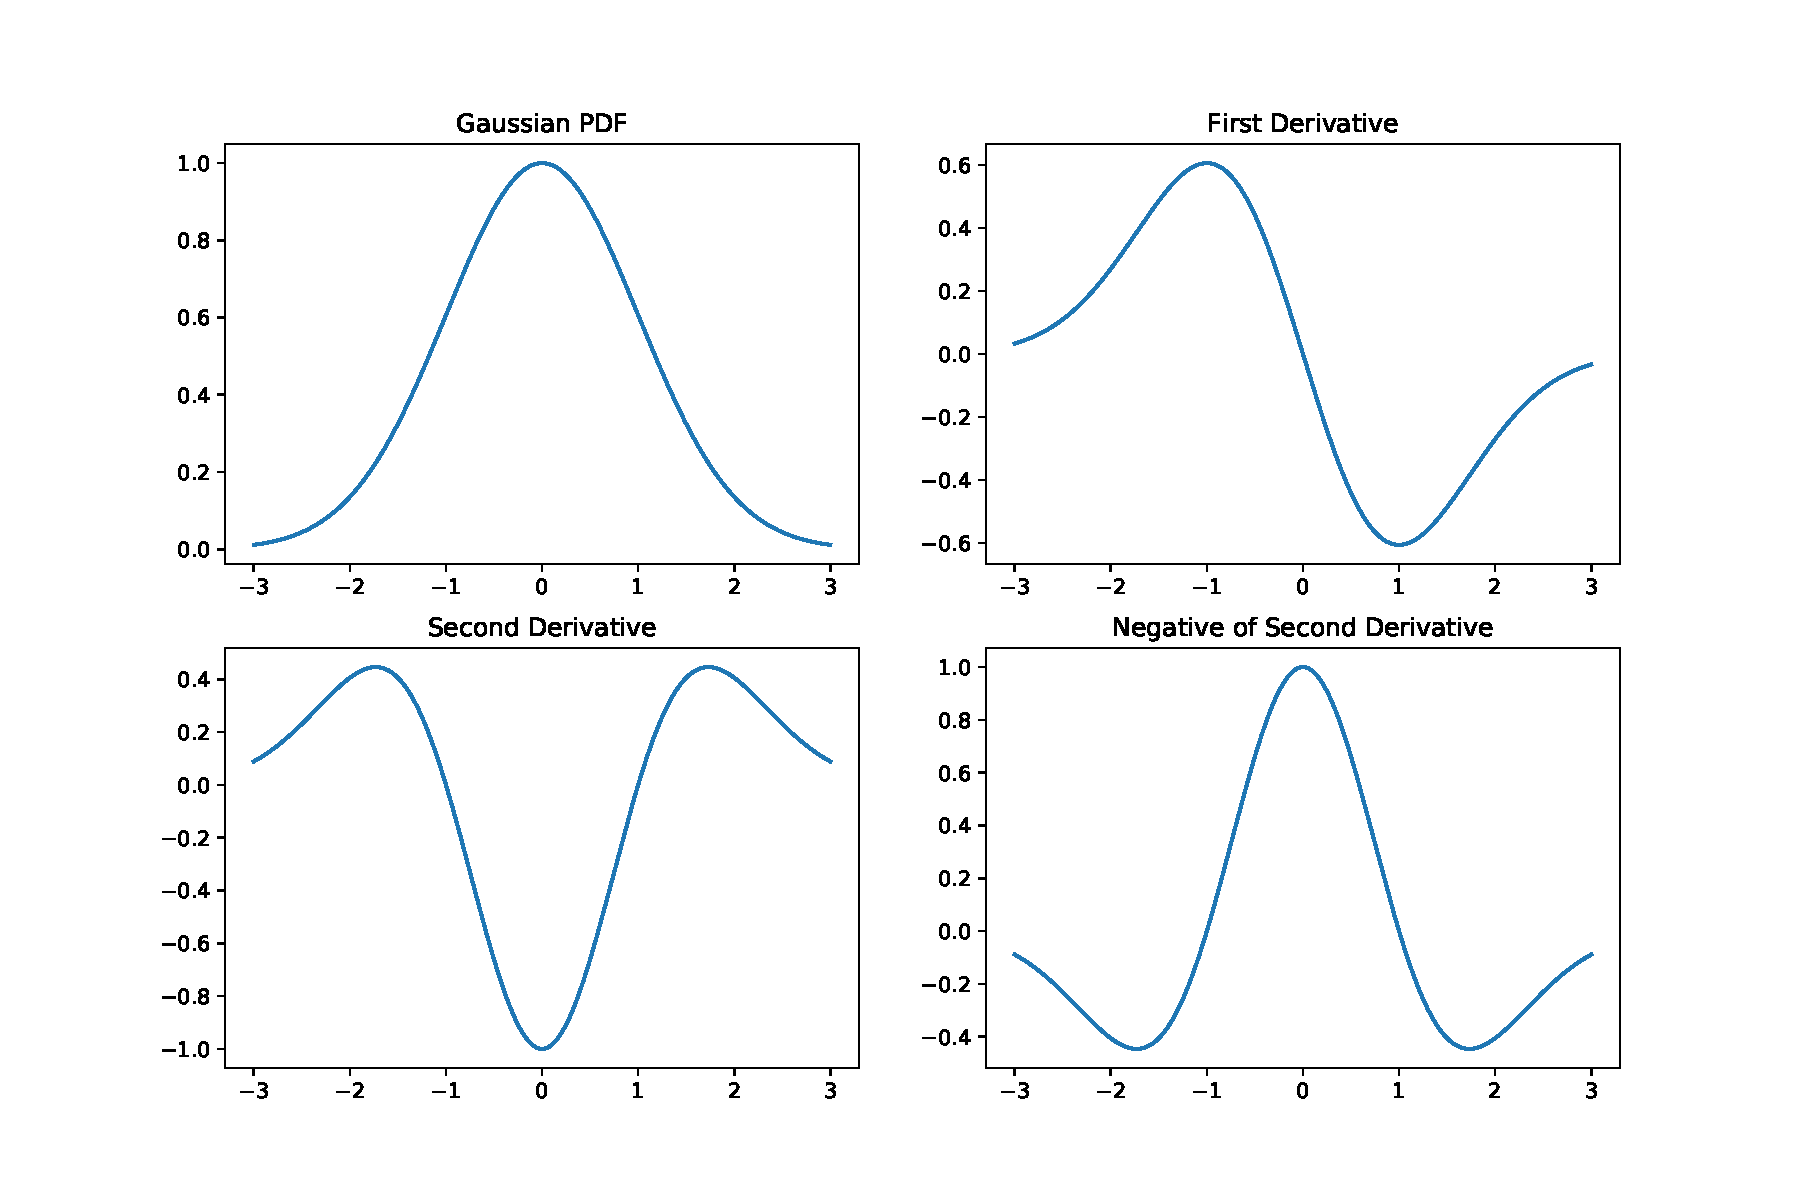
\includegraphics[width=\textwidth]{figs/mexican_hat_gaussian}
	\caption{Construction of Mexican Hat Filter from Gaussian (1D Example)\label{fig:mexicanhat}}
\end{figure}
By taking second derivative of the Gaussian density, and taking negative we get the Mexican Hat filter (1D). Figure \ref{fig:mexicanhat} illustrates the process. Around the centre of this hat, we will see positive values, e.g. approx. from -1 to 1 in our example. And if we go beyond the threshold, ($> 1 \vee < -1$) the the filter has negative values. This makes this function perfect for the role of blob detector! The 2D case can be easily obtained by revolving the 1D Mexican hat around zero point. 

\subsubsection{Laplacian of Gaussian Filter (2-D Formal)} Suppose $G: \real^2 \rightarrow \real$ specifies a Gaussian density, then 
\begin{equation}
	(\operatorname{LoG}(x,y) = \, ) \, L(x, y) \triangleq \Delta G = \partial_{xx} G + \partial_{yy} G
\end{equation}
is the laplacian\footnote{Note: Laplacian operator is a second order differential operator in the 2D Euclidian space. It is defined as the divergence of the gradient of the function. In our case, the function is gaussian density. $\Delta \bf = \nabla^2 \bf = \nabla \cdot\nabla \bf $} of Gaussian. Now let's derive this. We start with the 2D gaussian density (assuming isotropic density, i.e. $\Sigma = \sigma I$), which is
\begin{equation}
	G(x, y) = \underbrace{\frac{1}{2\pi \sigma^2}}_{c\in \real} \exp \underbrace{\left\{ - \frac{x^2 + y^2 }{2\sigma^2} \right\}}_{f(x,y)} = c e^{f(x,y)}
\end{equation}
Then,
\begin{align}
	\partial_x G = c \partial_x f e^{f(x,y)} \quad \implies \quad \partial_{xx} G &= c\left( \partial_{xx}f e^{f(x, y)} + \partial_x f\partial_x f e^{f(x,y)} \right) \\
	&= c \left( - \frac{1}{\sigma^2} e^{f(x,y)} + \frac{x^2}{\sigma^4} e^{f(x,y)} \right) \\
	&= c \left( \frac{x^2 - \sigma^2}{\sigma^4} \right) e^{f(x, y)}
\end{align}
and similarly, 
\begin{equation}
	\partial_{yy} G = c\left( \frac{y^2 - \sigma^2}{\sigma^4}\right)e^{f(x, y)} 
\end{equation}
then arrive at our final form 
\begin{align}
	L(x, y) 
	&= c \left( \frac{x^2 - \sigma^2}{\sigma^4} \right) e^{f(x, y)} + c\left( \frac{y^2 - \sigma^2}{\sigma^4}\right)e^{f(x, y)} \\
	&= \frac{1}{\pi \sigma^4} \left( \frac{x^2 + y^2}{2\sigma^2} - 1\right) \exp\left\{ - \frac{(x^2 + y^2)}{2\sigma^2} \right\}
\end{align}
The above final result will give us the inverse Mexican Hat ($\real^2 \rightarrow \real$). 

\subsubsection{LoG and Derivative of Gaussian wrt Variance} Recall that 
\begin{equation}
	\operatorname{LoG} (x, y)  = \frac{1}{\pi \sigma^4} \left( \frac{x^2 + y^2}{2\sigma^2} - 1\right) \exp\left\{ - \frac{(x^2 + y^2)}{2\sigma^2} \right\}
\end{equation}
and 
\begin{equation}
	G(x, y)=\underbrace{\frac{1}{2 \pi \sigma^{2}}}_{c \in \mathbb{R}} \exp \underbrace{\left\{-\frac{x^{2}+y^{2}}{2 \sigma^{2}}\right\}}_{f(x, y)}=c e^{f(x, y)}
\end{equation}
clearly they look similar to one another. Now we want to find how they are connected mathematically. Staring at the equation, let's start with making them look them by cancelling and constants in front. We have
\begin{align}
	\operatorname{LoG}(x,y) 
	&= G(x,y,\sigma) \frac{2\pi\sigma^2}{\pi\sigma^4} \left( \frac{x^2 + y^2}{2\sigma^2} - 1\right) \\
	&= G(x, y) \frac{1}{\sigma^{2}}\left(\frac{x^{2}+y^{2}}{\sigma^{2}}-2\right)
\end{align}
We can also derive that \note{add derivation to this, homework. }
\begin{equation}
	\frac{\partial G}{\partial \sigma}=\frac{1}{\sigma}\left(\frac{\left(x^{2}+y^{2}\right)}{\sigma^{2}}-2\right) G(x, y, \sigma)
\end{equation}
but wait! The above two equations look more than ``just similar'', in fact
\begin{equation}
	\partial_\sigma G = \sigma\operatorname{LoG}(x, y) = \sigma \Delta G(x, y) \label{eq:derivative of gaussian wrt sigma}
\end{equation}

\subsubsection{Difference of Gaussians\label{sec:difference of gaussians}}
By definition, the difference of gaussians is calculated as
\begin{align}
	\operatorname{DoG} (x, y, \sigma, k) 
	&= G(x, y, \sigma) - G (x, y, k\sigma) \\
	&= \frac{1}{2\pi\sigma^2}\exp\left\{ - \frac{x^2 + y^2}{2\sigma^2} \right\} - \frac{1}{2\pi k^2\sigma^2}\exp\left\{ - \frac{x^2 + y^2}{2k^2\sigma^2} \right\}
\end{align}
Then, 
\begin{align}
	\frac{-1}{k - 1} \operatorname{DoG} 
	&= \frac{G(x, y, \sigma) - G(x, y, k\sigma)}{\sigma - k \sigma} \sigma \\
	&\overset{k \rightarrow 1}{\approx} \frac{\partial G}{\partial \sigma}\cdot \sigma
\end{align} 
Recall from Equation \ref{eq:derivative of gaussian wrt sigma}, then we know
\begin{equation}
	\operatorname{DoG} \approx (1 - k) \sigma \frac{\partial G}{\partial \sigma} = (1 - k) \sigma^2 \Delta G(x, y). 
\end{equation}

\subsubsection{Approximating Laplacian of Gaussian w/ Difference of Gaussians}
To see how the above two sections relate, we will need one example. Suppose we have an image $I(x,y)$, $\sigma(s) = 2^s$, $R(x,y,\sigma) = \left( G(x,y,\sigma) \ast I(x,y) \right)$. Now let's take the derivative of $R$ with respect to the scale parameter $s$ here, 
\begin{align}
	\frac{\partial R}{\partial s} 
	&= \frac{\partial G}{\partial s} \ast I(x,y) \\
	&= \log 2 \sigma(s) \left( \frac{\partial G}{\partial \sigma} \ast I(x,y)\right) \\
	&= \log 2 \sigma^2 \Delta G(x,y) \ast I(x,y)
\end{align}
Now notice the final result from Section \ref{sec:difference of gaussians} Difference of Gaussians contains a similar filter as what we just derived. Scientist uses difference of gaussians as approximation for laplacian of gaussian filter. 

\paragraph{But Why Isn't LoG Good Enough?} The LoG filter is a non-separable one, and things get especially bad when we need a filter of large size. The laplacian of gaussian filter however, is a lot faster in terms of computation time since it is separable. 

\subsubsection{Applying Laplacian of Gaussian 1-D}
When we try to use laplacian of gaussian to detect blob, we first convolve the input signal with the LoG with some arbitrary $\sigma$. Then we gradually increase the sigma, and find extremes that are scale invariant in terms of $\sigma$. 

\subsubsection{Characteristic Scale} We define the characteristic scale as the scale that produces peak (min / max) of the Laplacian response. This means that to detect a blob of certain size, we will need a Laplacian of Gaussian of a certain ``scale'' - the characteristic scale!

\subsubsection{Applying Laplacian of Gaussian 2-D}
\begin{figure}[H]
	\center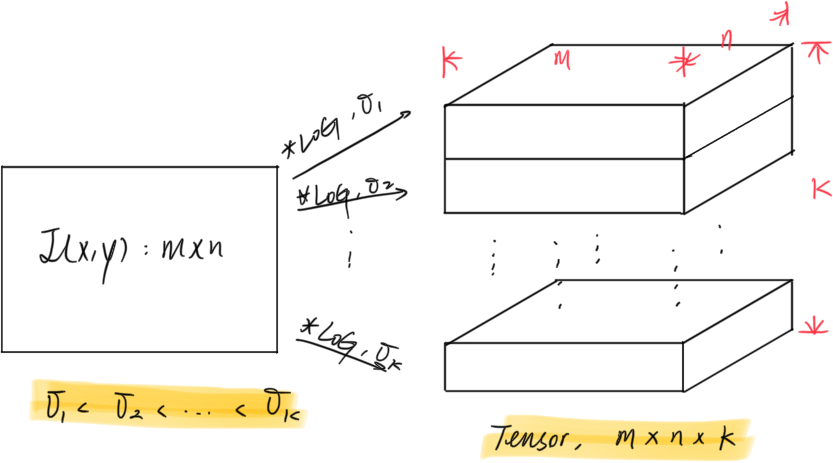
\includegraphics[width=0.85\textwidth]{figs/2d_log}
	\caption{Using Laplacian of Gaussian to find interest points in 2D case (images). Interest points are local maxima in both position and scale. \label{fig:2d_log}}
\end{figure}
Applying Laplacian of Gaussian in 2D image case is similar to the 1D case presented earlier, just this time we have an array of output maps (really a tensor). Figure \ref{fig:2d_log} illustrates the input and output. The interest points that we want to find are local maxima in both position and scale, i.e. interest points are consistent along vertical direction in the output tensor. 

\subsubsection{Lowe's Difference of Gaussian}
First compute a Gaussian image pyramid, and then compute the Difference of Gaussians
\begin{equation}
	D(x, y, \rho)=I(x, y) *(G(x, y, k \rho)-G(x, y, \rho))
\end{equation}
for $\rho=\left\{\sigma, k \sigma, k^{2} \sigma, \ldots, k^{s-1} \sigma\right\}$ where $k = 2^{1/s}$. The application process is quite similar to the LoG one we discussed above, we will need to compute
\begin{align}
	&I_s = I * G_{k^s \sigma} \\
	&\quad \vdots \\
	&I_2 = I * G_{k^2\sigma} \\
	&I_1 = I * G_{k^1\sigma} \\
	&I_0 = I * G_{k^0\sigma}
\end{align}
Then we compute their differences (element-wise). There should be $s$ difference maps, i.e. $I_1 - I_0, I_2 - I_1, ...$. Once we are done with the current scale, we will do it for the next one. (this is why we need the gaussian pyram id in the first place.) Finally, we find local maxima in scale, and do a bit of pruning of bad maxima.\footnote{Look over every $x$ and $y$, what is the highest response in the scale space? We will keep all points with response greater than a certain threshold. } We are done! 

\subsubsection{Other Interest Point Detectors}
\begin{itemize}
	\item Lindeberg: Laplacian of Gaussian
	\item Lowe: DoG (Typically called the SIFT interest point detector)
	\item Mikolajczyk \& Schmid: Hessian / Harris laplacian / Affine
	\item Tuyttelaars \& Van Gool: EBR and IBR
	\item Matas: MSER
	\item Kadir \& Brady: Salient Regions
\end{itemize}


\section{Scale Invariant Feature Transform (SIFT)}
%\paragraph{Process of Identifying and Matching Interest Points}
%\begin{itemize}
%	\item Detection: Identify the interest points
%	\item Description: Extract a feature descriptor around each interest point
%	\item Matching: Determine correspondence between descriptors in two views
%\end{itemize}
\subsection{Step 1: Difference of Gaussians as Feature Detector}
The first step is the same as described in section Lowe's Difference of Gaussian. First compute a Gaussian image pyramid, and then compute the Difference of Gaussians
\begin{equation}
	D(x, y, \rho)=I(x, y) *(G(x, y, k \rho)-G(x, y, \rho))
\end{equation}
for $\rho=\left\{\sigma, k \sigma, k^{2} \sigma, \ldots, k^{s-1} \sigma\right\}$ where $k = 2^{1/s}$. The application process is quite similar to the LoG one we discussed above, we will need to compute
\begin{align}
	&I_s = I * G_{k^s \sigma} \\
	&\quad \vdots \\
	&I_2 = I * G_{k^2\sigma} \\
	&I_1 = I * G_{k^1\sigma} \\
	&I_0 = I * G_{k^0\sigma}
\end{align}
Then we compute their differences (element-wise). There should be $s$ difference maps, i.e. $I_1 - I_0, I_2 - I_1, ...$.

\subsection{Step 2: Extracting Feature Points}
For each key-point, we take the Gaussian-blurred image at corresponding scale $\rho$. Notice that this information needs to be stored as a pair. We will need this in the following steps. 

\subsection{Step 3: Gradient Magnitude and Orientation}
Compute the gradient magnitude and the orientation in neighbourhood of each keypoint proportional to the detect scale. To achieve so, we first blur the image with gaussian wth respective $\rho$, 
\begin{equation}
	I \ast G_\rho
\end{equation}
Then, compute, on a $16 \times 16$ neighbour around the key-point, the magnitude of gradients 
\begin{equation}
	|\nabla I(x, y)|=\sqrt{\left(\frac{\partial\left(I(x, y) * G_{\rho}\right)}{\partial x}\right)^{2}+\left(\frac{\partial\left(I(x, y) * G_{\rho}\right)}{\partial y}\right)^{2}}
\end{equation}
and the gradient orientation
\begin{equation}
	\theta(x, y)=\arctan \left(\frac{\partial I * G_{\rho}}{\partial y} / \frac{\partial I * G_{\rho}}{\partial x}\right)
\end{equation}

\subsection{Step 4: Dominant Orientation Extraction}
In this step, we wish to weigh gradients closer to the centre of the $16 \times 16$ patch higher. We can achieve so by element-wisely scale the gradient magnitudes according to a gaussian density
\begin{equation}
	\nabla I(x, y) \mid \cdot G_{1.5 \rho}(d)
\end{equation}
then we compute a histogram of gradient orientations, each bin covers $10\deg$. The orientation giving the peak in the histogram is the key point's orientation. 

\subsection{Step 5: Computing the Feature Vector}
Compute a 128 dimensional descriptor: $4 \times 4$ grid, each cell is a histogram of 8 orientation bins relative to dominant orientation. Each descriptor has 
\begin{equation}
	P_i = (x_i, y_i, \rho_i, \vartheta_i ) \quad\text{and} \quad f_i = ... \in \real^{128}
\end{equation}
where $x_i, y_i$ marks the location, $\rho_i$ marks scale, $\vartheta_i$ is the orientation and $f_i$ is the feature vector. This step is a bit abstract and hard to follow, let's dive deeper. Figure \ref{fig:compute feature vector SIFT} illustrates the process. Each $4 \times 4$ component in the original $16 \times 16$ window contributes to the 128 dim\footnote{The original $16 \times 16$ grid is now treated as a $4 \times 4$, since each $4 \times 4$ subunit is now treated as one entity. There is one 8 bin histogram in each $4 \times 4$ grid, and thus we have $4 \times 4 \times 8 = 128$ bin values in total. } vector as one unit, via a 8 bin histogram. 
\begin{figure}[H]
	\center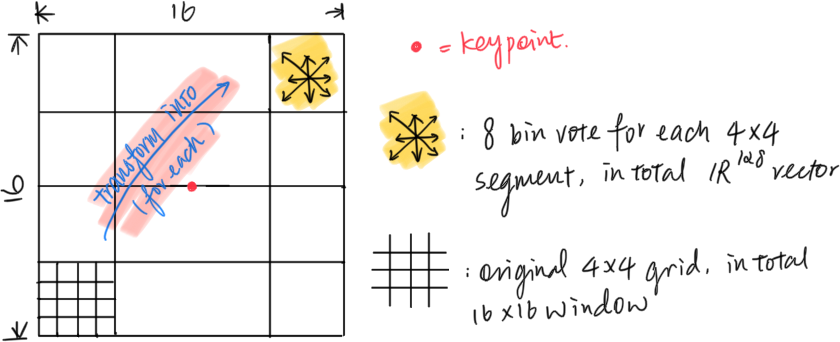
\includegraphics[width=0.9\textwidth]{figs/compute_feature_vector_SIFT}
	\caption{The $4 \times 4$ grid 8 bin vote transformation process. \label{fig:compute feature vector SIFT}}
\end{figure}

\subsubsection{Achieving Rotation Invariance} Our method as it is now is rotation dependent, i.e. if I rotate the original input image, everything will change. But how can we make it rotation invariant? At this point, we already have the dominant orientation from Step 4, so we just make the 8 bins based on the dominant orientation direction. 

\subsubsection{Achieving Illumination Independence} To achieve this, we just need to use some thresholding. Suppose we have an feature vector \texttt{f1} $\in \real^{128}$, then\footnote{I am using pseudo-code here just to make everything easier... }
\begin{equation}
	\texttt{f2[j] = f1[j] > thres ? thres : f1[j], for each j }
\end{equation}
Finally, we need to normalize \texttt{f2}, 
\begin{equation}
	\texttt{f = (f2 .- mean(f2)) ./ normL2(f2)}
\end{equation}

\subsection{Properties of SIFT}
SIFT is invariant to
\begin{itemize}
	\item scale, and 
	\item rotation
\end{itemize}
SIFT is partially invariant to 
\begin{itemize}
	\item Illumination changes (sometimes even day vs night) 
	\item Camera viewpoint ( up to about 60 deg of freedom of out of plane rotation.  
	\item Occlusion, clutter \note{why?}
\end{itemize}
Also it is important that SIFT is fast and efficient, can be run in real time! There are also a lot of code available :D. 


\subsection{PCA-SIFT} 
The dimensionality of SIFT is pretty high, we need 128 dimensions for each key point. We can try to reduce he dimensionality using linear dimensionality reduction such as Principle Component Analysis (PCA). We can reduce the dimensionality of each descriptor to 10 or so with PCA. 


\subsection{Matching Local Descriptors}
So far, we have talked about SIFT, which computes a bunch of local descriptors for interest points. But now we want to match the features between pairs of images. Ideally, a match is a correspondence between a local part of the object on one image to the same local part of the object in another image. The na\"ive approach on this is to brute force compare all possible pairs of interest points detected in two images, and see if we have a match by computing a distance metric such as Euclidean distance. But can we rely solely on this min Euclidean distance criteria as the indicator of a match? There will be cases that several close matches exist, which essentially means that the system is not confident on one choice. To address this, we introduce the ratio
\begin{equation}
	\phi_{i}=\frac{\left\|f_{i}-f_{i}^{\prime *}\right\|}{\left\|f_{i}-f_{i}^{\prime **}\right\|} = \frac{{\text {Distance to closest}}}{{\text {Distance to second closest}}}
\end{equation}
where $f_i^{\prime \ast}$ is the closest and $f_i^{\prime \ast\ast}$ is the second closest. If $\phi_i$ is small enough, then we have a reliable match. Otherwise if $\phi_i$ is large, then the system is unconfident. Notice that
\begin{itemize}
	\item High threshold introduces false positives, i.e. incorrect matches being returned, while
	\item Low threshold results in false negatives, i.e. too many correct matches being missed. 
\end{itemize}
Typically, we pick $\phi_i < 0.8 $

\section{Planar Objects Matching in New Viewpoints}
\subsection{Review: Linear Transformations}
Linear transformations / linear maps are combinations of Scale, rotation, shear and mirror. A transformation $T$ maps from one vector space into another one, and $T: V\rightarrow W$ is linear iff $\forall \bu, \bv \in V, k \in \real$
\begin{itemize}
	\item $T(\bu + \bv) = T(\bu) + T(\bv) \in W$
	\item $T(k\bu) = kT(\bu)$
\end{itemize}
In our context of image, and in our task of finding the transformation between viewpoint changes of images, we will be dealing with $2\times 2$ images, and the linear map will be achieved via a matrix multiplication 
\begin{equation}
	\left[\begin{array}{l}
		x^{\prime} \\
		y^{\prime}
		\end{array}\right]=\left[\begin{array}{ll}
		a & b \\
		c & d
		\end{array}\right]\left[\begin{array}{l}
		x \\
		y
	\end{array}\right]
\end{equation}
And there are several canonical transformation matrices (form) that get used often
\paragraph{Scaling Matrix}
\begin{equation}
	\left[\begin{array}{l}
		x^{\prime} \\
		y^{\prime}
		\end{array}\right]=\left[\begin{array}{ll}
		s_1 & 0 \\
		0 & s_2
		\end{array}\right]\left[\begin{array}{l}
		x \\
		y
	\end{array}\right]
\end{equation}

\paragraph{Rotation Matrix} Counter-clock wise rotation $\theta$ radian of the original vector space. 
\begin{equation}
	\left[\begin{array}{l}
		x^{\prime} \\
		y^{\prime}
		\end{array}\right]=\left[\begin{array}{ll}
		\cos \theta & -\sin\theta \\
		\sin\theta & \cos\theta
		\end{array}\right]\left[\begin{array}{l}
		x \\
		y
	\end{array}\right]
\end{equation}

\paragraph{Shear Matrix} `distorts' rectangles into parallelograms. 
\begin{equation}
	\left[\begin{array}{l}
		x^{\prime} \\
		y^{\prime}
		\end{array}\right]=\left[\begin{array}{ll}
		1 & \lambda\, | \,0 \\
		0\, | \,1 & 1
		\end{array}\right]\left[\begin{array}{l}
		x \\
		y
	\end{array}\right]
\end{equation}

\paragraph{Mirror Matrix} Let
\begin{equation}
	A = \begin{bmatrix}
		-1 & 0 \\ 0 & -1
	\end{bmatrix} \quad B = \begin{bmatrix}
		-1 & 0 \\ 0 & 1 
	\end{bmatrix} \quad C = \begin{bmatrix}
		1 & 0 \\
		0 & -1
	\end{bmatrix}
\end{equation}
then, $A$ mirrors both $x$ and $y$ directions, and $B, C$ mirrors only $x$ or only $y$ respectively. 

\subsubsection{Properties of Linear Transformations}
\begin{itemize}
	\item Origin always maps to origin, and 
	\item lines always map to lines, and 
	\item parallel lines remain parallel, and 
	\item ratios are preserved, and 
	\item closed under composition, meaning that we can collapse a serial of matrix together before applying it. Often, this is computationally more efficient. 
\end{itemize}

\subsection{Affine Transformations}
So far, we've discussed linear transformations, which only accounts for transformation not translation. To address, we introduce the affine transformation, which takes the general form of 
\begin{equation}
	\left[\begin{array}{l}
		x^{\prime} \\
		y^{\prime}
		\end{array}\right]=\left[\begin{array}{ll}
		a & b \\
		c & d
		\end{array}\right]\left[\begin{array}{l}
		x \\
		y
		\end{array}\right]+\left[\begin{array}{l}
		e \\
		f
	\end{array}\right] = \left[\begin{array}{lll}
		a & b & e \\
		c & d & f
		\end{array}\right]\left[\begin{array}{l}
		x \\
		y \\
		1 
	\end{array}\right]
\end{equation}

\subsubsection{Properties of Affine Transformations}
\begin{itemize}
	\item {\color{Orange} Origin does not necessarily map to origin. }
	\item Lines map to lines, and
	\item parallel lines remain parallel
	\item ratios are preserved, and 
	\item closed under composition, and 
	\item rectangles go parallelograms
\end{itemize}

\subsubsection{Approximating View Point Changes}
Affine transformation approximates viewpoint changes for roughly planar objects and roughly orthographic cameras. 

\subsubsection{Computing the Affine Transformation}
Let $(x_i,y_i)$ be a point on the reference (model) image and $x_i', y_i'$ its match in the test image. An affine transformation $A$ maps $(x_i,y_i)$ to $(x_i',y_i')$:
\begin{equation}
	\left[\begin{array}{l}
		x_{i}^{\prime} \\
		y_{i}^{\prime}
		\end{array}\right]=\left[\begin{array}{lll}
		a & b & e \\
		c & d & f
		\end{array}\right]\left[\begin{array}{l}
		x_{i} \\
		y_{i} \\
		1
	\end{array}\right]
\end{equation}
where the matrix with elements $a, b, ..., f$ is a unknown matrix. This system gives us 2 equations, but we have 6 unknowns to solve for. To address, we can rewrite this into a simple linear system. (still 2 equations with 6 unknowns)
\begin{equation}
	\begin{bmatrix}
		x_i & y_i & 0 & 0 & 1 & 0 \\
		0 & 0 & x_i & y_i & 0 & 1
	\end{bmatrix} \begin{bmatrix}
		a \\ b \\ c \\ d \\ e \\ f 
	\end{bmatrix} = \begin{bmatrix}
		x_i' \\ y_i'
	\end{bmatrix}
\end{equation}
but the catch is that we have more than one match! and for each match we have two equations. We can stack all the equations up\footnote{Vertically stack the matrices} and make it a bigger system, still with just 6 unknowns. Let's call this stacked system as 
\begin{equation}
	P\ba = \bp'
\end{equation}
Notice that here it suffices to have three matching points to solve for the affine transformation. If we have three matches, then computing $A$ is really easy:
\begin{equation}
	\ba = P^{-1}\bp'
\end{equation}
However, the more matching points data we have, the more reliable it will be, and in this case, we do the least squares estimation
\begin{equation}
	\underset{a, b, ..., f}{\operatorname{min}} \norm{P\ba - \bp'}_2^2
\end{equation} 
which has a closed form solution
\begin{equation}
	\ba = (P^\top P) ^{-1} P^\top \bp'
\end{equation}
where $(P^\top P) ^{-1} P^\top$ is called Moore-Penrose Pseudo-inverse. 

\subsubsection{RANdom SAmple Consensus (RANSEC)}
In previous sections, we assumed that there will be good correspondence between points. However, in reality, this might not be true, and we might suffer from outliers. In particular, least square estimation is very sensitive to outliers. RANSAC is here to the rescue. The approach is quite simple, and is as follows:
\begin{itemize}
	\item Take the minimal number of points to compute what we want. In a Simple Linear Regression (SLR) line example, two point. And in our affine example of matching two images, three matches. 
	\item By ``take'' we mean choose at random from all points
	\item fit a line to the selected pair of points 
	\item count the number of all points that agree with\footnote{within some $\delta$ neighbourhood of the line} the line: calling them inliers.
	\item repeat this many times, remember the number of inliers for each trial, and the respective points selected for the generation of that specific line
	\item among several trials, select the one with the largest number of inliers. 
\end{itemize}

\paragraph{How many iterations?}  
\begin{itemize}
	\item Suffience number of trials $S$ must be tried
	\item Let $p$ be the probability that any given correspondence is valid and $P$ be the total probability of success after $S$ trials. 
	\item The likelihood in one trial that all $k$ random samples are inliers is $p^k$, then
	\item At least one one the $k$ points is an outlier has probability $(1 - p^k)$,
	\item All $S$ trials are bad has probability $(1 - p^k)^S$, then
	\item the probability of a least one is good is
		\begin{equation}
			P = 1 - (1 - p^k)^S
		\end{equation}
	\item and it is possible to solve 
		\begin{equation}
			S = \frac{\log (1 - P)}{\log (1 - p^k)} 
		\end{equation}
		where $P \uparrow \implies S\uparrow$, and $p\downarrow \implies S\uparrow$, and $k \uparrow \implies S\uparrow$
\end{itemize}

%\section{Machine Learning Vision}
%This section is skipped. 

\section{Camera Models}
Images are 2D projections of the real world scene, it captures two kinds of information
\begin{itemize}
	\item Geometric: positions, points, lines, curves, etc
	\item Photometric: intensity, color
\end{itemize}
There is a complex 2D - 3D relationship between the 2D image captured by an camera and the actual scene which is in 3D. We use the camera model to approximate these relationships. We will discuss how are 3D primitives projected onto the image plane. We can do this using a linear 3D to 2D projection matrix. 

\subsection{Pinhole Camera Model}
The distance from the camera pinhole to the image plane (which has the upside down, left-side right image projected) is called the focal length, denoted $f$. A virtual image plane is between the camera pinhole and the object in the world. It will be exactly focal length away from the camera centre, and it will have the exact same sized image as the image plane. (except this one is not upside down and left-side right. ) It is easier to consider this plane. Now the goal is to find how the object in the world projects to the (virtual) image plane. 

\subsection{Camera / Image Coordinate System}
We define the camera pinhole as the origin $\bzero \in \real^3$, it is called the optical centre. We use the right hand rule for specification of axis positive orientations. That is, from the perspective of the camera, towards left means positive in $X$ direction, and upwards means positive in $Y$ direction and further away from the camera (increase in depth of field) corresponds to positive direction in $Z$. 

The $Z$ axis is given the name of \textbf{Optical Axis} or \textbf{Principal Axis}. It is orthogonal to the (virtual) image plane between the object in the world and the camera centre. The camera coordinate axes $X, Y$ are parallel to the image plane. The principal point $\bp$ denotes the point where the principal axis intersects with the image plane. Note that $\norm{\bp}$ is equal to the focal length. 

We denote the image axes with $x$ and $y$. An image we see is of course represented with these axes. We call this an image coordinate system. 

\subsection{Projection}
Suppose we have a point $Q\in\real^3 = (\bx, \by, \bz)^\top$. (suppose that it $\bz > f$) Then, using similar triangles (actually 3D similar triangles in this case), we know that this $Q$ will appear on the virtual image plane at
\begin{equation}
	\left(\frac{f \cdot \bx}{\bz}, \frac{f \cdot \by}{\bz}, f\right)^{\top}
\end{equation}
The notion above is relative to the principal point $\bp$, but on a 2D projection the depth information is extraneous, and we can disregard it. We do so by essentially moving the origin to $(0, 0)$ in the image. Let $\bp$ have coordinates $(p_x, p_y)$ on the image plane in terms of the image coordinate system, then the projection is
\begin{equation}
	\left(\frac{f \cdot \bx}{\bz}+p_{x}, \frac{f \cdot \by}{\bz}+p_{y}, 0\right)^{\top}
\end{equation}
then the depth dimension is no longer useful and we have the actual projection onto the 2D image plane by throwing the last coordinate, i.e. 
\begin{equation}
	Q = (\bx, \by, \bz)^\top \rightsquigarrow q = \left(\frac{f \cdot \bx}{\bz}+p_{x}, \frac{f \cdot \by}{\bz}+p_{y}\right)^{\top} \label{eq:perspective projection original}
\end{equation}
Notice that this is not a linear transformation, since we have a division of $\bz$ in in the new coordinate. (it is linear in terms of $1/\bz$ but not in terms of $\bz$). The problem now is how I can make this $\rightsquigarrow$ happen, but linearly. 

We will use homogeneous coordinates (aka projective coordinates), which simply append 1 to the vector. For a 2D position $(x, y)$, it becomes $(x, y, 1)$. Similarly for 3D positions, which will turn into a 4D vector. 

\begin{mdframed}
	\paragraph{Side Note: Homogeneous Coordinates}
A brief summarization of what homogeneous coordinates are ... borrowed from \url{https://en.wikipedia.org/wiki/Homogeneous_coordinates#Notation}
\begin{itemize}
	\item Any point in the projective plane is represented by a triple $(X, Y, Z)$, called the homogeneous coordinates or projective coordinates of the point, where $X, Y$ and $Z$ are not all 0.
	\item The point represented by a given set of homogeneous coordinates is unchanged if the coordinates are multiplied by a common factor. 
	\item Conversely, two sets of homogeneous coordinates represent the same point if and only if one is obtained from the other by multiplying all the coordinates by the same non-zero constant.
	\item When Z is not 0 the point represented is the point (X/Z, Y/Z) in the Euclidean plane.
	\item When Z is 0 the point represented is a point at infinity.
	\item Note that the triple (0, 0, 0) is omitted and does not represent any point. The origin is represented by (0, 0, 1).
\end{itemize}
\end{mdframed}

In homogeneous coordinates, scaling doesn't affect anything, i.e. $(x, y, 1)$ is congruent with $(wx, wy, w)$ for $w\in\real \neq 0$. This fits the our projection line model, since all points along a projection line map to a single point $\bq$ on the image. We can write what we want in Equation \ref{eq:perspective projection original} homogeneous coordinates, 
\begin{equation}
	Q=(\bx, \by, \bz)^{\top} \quad \rightarrow \quad q=\left[\begin{array}{c}
		\frac{f \cdot \bx}{\bz} + p_{X} \\
		\frac{f \cdot \by}{\bz} + p_{y} \\
		1
		\end{array}\right] \sim\left[\begin{array}{c}
		f \cdot \bx + \bz \cdot p_{x} \\
		f \cdot \by + \bz \cdot p_{y} \\
		\bz
	\end{array}\right]
\end{equation}
and then we can write this as a matrix multiplication
\begin{equation}
	Q = \begin{bmatrix}
		\bx, \by, \bz
	\end{bmatrix}^\top \rightarrow 
	\begin{bmatrix}
		f\bx + \bz p_x \\
		f\by + \bz p_y \\
		\bz
	\end{bmatrix} = \begin{bmatrix}
		f & 0 & p_x \\
		0 & f & p_y \\
		0 & 0 & 1
	\end{bmatrix} \begin{bmatrix}
		\bx \\ \by \\ \bz
	\end{bmatrix}
\end{equation}
where we denote 
\begin{equation}
	K = \begin{bmatrix}
		f & 0 & p_x \\
		0 & f & p_y \\
		0 & 0 & 1
	\end{bmatrix}
\end{equation}
is called the \textbf{camera calibration matrix} or \textbf{intrinsic parameter matrix}. The parameters in $K$ are called \textbf{internal camera parameters}.

Finally,
\begin{equation}
	K \begin{bmatrix}
		\bx, \by, \bz
	\end{bmatrix}^\top = \begin{bmatrix}
		wx \\ wy \\ w
	\end{bmatrix} \rightarrow q = \begin{bmatrix}
		x \\y 
	\end{bmatrix} \implies \begin{cases}
		x = \frac{f\bx}{\bz} \cdot p_{x} \\
		y = \frac{f\by}{\bz} \cdot p_{y}
	\end{cases}
\end{equation}

\subsection{Camera Calibration Matrix}
We presented that the Camera Calibration Matrix is denoted as $K$, and has values (this first formulation assumes square pixels)
\begin{equation}
	K = \begin{bmatrix}
		f & 0 & p_x \\
		0 & f & p_y \\
		0 & 0 & 1
	\end{bmatrix}
\end{equation}
It can be a little more complicated, as pixels may not be square, (different focal length in $x$ and $y$ direction, denoted by $f_x$ and $f_y$ respectively.) 
\begin{equation}
	K = \begin{bmatrix}
		f_x & 0 & p_x \\
		0 & f_y & p_y \\
		0 & 0 & 1
	\end{bmatrix}
\end{equation}
and there might be a skew angle $\theta$ between $x$ and $y$ image axis
\begin{equation}
	K = \begin{bmatrix}
		f_x & -f_x\cot \theta & p_x \\
		0 & f_y / \sin\theta & p_y \\
		0 & 0 & 1
	\end{bmatrix}
\end{equation}

\subsection{Projection Properties}
\subsubsection{Many to One Projection}
In the case of many to one projection, any points along same ray map to same point in image. Particularly,
\begin{itemize}
	\item Points always map to points, and 
	\item lines usually, though not always, map to lines. (A line going through the principle point maps to a point instead!) \note{wait shouldn't this be: principle axis maps to a point? } 
	\item planes usually, though not always, map to planes. (A plane going through principal point projects to line)
\end{itemize}

\subsubsection{Vanishing Point}
Parallel lines converge at a vanishing point. Each different direction in the world has its own vanishing point. All lines in the same direction in 3D intersect at the same vanishing point. Notice that this vanishing point is not necessarily inside the virtual image plane, but parallel lines in the world always converge to the same vanishing point. 

A line that passes through $V$ with direction $D$ can be written as
\begin{equation}
	X = V + tD\quad t \in\real
\end{equation}
Then if we project it, we have
\begin{equation}
	\left[\begin{array}{c}
			w x \\
			w y \\
			w
		\end{array}\right]=K X=\left[\begin{array}{ccc}
			f & 0 & p_{x} \\
			0 & f & p_{y} \\
			0 & 0 & 1
		\end{array}\right]\left[\begin{array}{c}
			V_{x}+t D_{x} \\
			V_{y}+t D_{y} \\
			V_{z}+t D_{z}
		\end{array}\right]=\left[\begin{array}{c}
			f V_{x}+f t D_{x}+p_{x} V_{z}+t p_{x} D_{z} \\
			f V_{y}+f t D_{y}+p_{y} V_{z}+t p_{y} D_{z} \\
			V_{z}+t D_{z}
	\end{array}\right]
\end{equation}
then we move infinitely far from the camera by taking $t \rightarrow \infty$ and compute $x, y$\footnote{when $t \rightarrow \infty$, $fV_x, p_xV_z, V_z$ are all constants, and thus are small numbers. They don't matter. Same for the $y$ ones. }
\begin{equation}
	x=\lim _{t \rightarrow \infty} \frac{f V_{x}+f t D_{x}+p_{x} V_{z}+t p_{x} D_{z}}{V_{z}+t D_{z}}=\frac{f D_{x}+p_{x} D_{z}}{D_{z}}
\end{equation}
\begin{equation}
	y=\lim _{t \rightarrow \infty} \frac{f V_{y}+f t D_{y}+p_{y} V_{z}+t p_{y} D_{z}}{V_{z}+t D_{z}}=\frac{f D_{y}+p_{y} D_{z}}{D_{z}}
\end{equation}
Importantly, this solution is independent of $V$, meaning that all lines with direction $D$ go to this point. 

\paragraph{*} Vanishing point can also be computed in another way. If we translate line with direction $D$ to the camera centre, the the intersection of the line with the virtual image plane is the vanishing point corresponding to direction $D$!

We must also remember that vanishing points might not exist. In cases where lines parallel to image plane are also parallel in the image, they intersect at infinity! Also, for lines in the same 3D plane, the vanishing points lie on a line. We all it a vanishing line. The vanishing line for the ground plane is a horizon line. 

\subsection{Camera Extrinsics}
The world is not described in camera coordinates, it is described by yet another system which is $(X_{world}, Y_{world}, Z_{world})$. The camera is placed at location $c$. Suppose our point of interest is $Q$, then clearly $Q - c$ makes the position relative to the camera. But the problem is what is $Q$ in camera's coordinate system? 

Suppose $u, v, w$ are three orthogonal directions of camera in room coordinate system. (much like a basis for movements of the camera.) Our goal is to have a rotation matrix $R$, that can take us from the world coordinate to the camera coordinate. Clearly the $R$ is such that $R \begin{bmatrix}
	u & v & w
\end{bmatrix} = I$ and $R R^\top = I$. 
Let 
\begin{equation}
	R = \begin{bmatrix}
		u^\top & v^\top & w^\top
	\end{bmatrix} \in\mat{3}{3}
\end{equation}
Then, $\begin{bmatrix}
	X' & Y' & Z'
\end{bmatrix}^\top$ in camera coordinates is
\begin{equation}
	\begin{bmatrix}
		X' \\ Y' \\ Z'
	\end{bmatrix} = R \left( \begin{bmatrix}
		X \\ Y \\ Z
	\end{bmatrix} - c \right) = \begin{bmatrix}
		R & -Rc
	\end{bmatrix}\begin{bmatrix}
		X \\ Y \\ Z \\ 1
	\end{bmatrix}
\end{equation}
where $\begin{bmatrix}
		X & Y & Z & 1
	\end{bmatrix}$ is in room / world coordinates. 

\subsection{Projection Equations}
The projection matrix $P$ models the culmulativeeffect of all intrinsic and extrinsic parameters. We use homogenous coordinates for 2D and 3D:
\begin{equation}
	q = \begin{bmatrix}
		ax \\ ay \\ a
	\end{bmatrix} = P \begin{bmatrix}
		X \\ Y \\ Z \\ 1
	\end{bmatrix}
\end{equation}
It can be computed as
\begin{equation}
\mathrm{P}=\underbrace{\left[\begin{array}{ccc}
		f & 0 & p_{x} \\
		0 & f & p_{y} \\
		0 & 0 & 1
	\end{array}\right]}_{\text {intrinsics } K} \underbrace{\left[\begin{array}{cccc}
		1 & 0 & 0 & 0 \\
		0 & 1 & 0 & 0 \\
		0 & 0 & 1 & 0
	\end{array}\right]}_{\text {projection }} \underbrace{\underbrace{\left[\begin{array}{cc}
	\mathrm{R}_{3 \times 3} & 0_{3 \times 1} \\
	0_{1 \times 3} & 1
	\end{array}\right]}_{\text {rotation }} \underbrace{\left[\begin{array}{cc}
	\mathrm{I}_{3 \times 3} & \mathrm{~T}_{3 \times 1} \\
		0_{1 \times 3} & 1
	\end{array}\right]}_{\text {translation }}}_{\begin{bmatrix}
		R  &  -c
	\end{bmatrix}}
\end{equation}
To get a point $q$ in the image plane, I need to compute
\begin{equation}
	P(X, Y, Z, 1)^\top
\end{equation}
where $P\in\mat{3}{4}$. This gives me a 3 by 1 vector. Now I divide all coordinates with the third coordinate (making the third coordinate equal to 1), and then drop the last coordinate. 

The projection matrix can be compactly written as 
\begin{equation}
	P = K \begin{bmatrix}
		R & -c
	\end{bmatrix}
\end{equation}
The (brutal) truth is in most cases you don't have $P$ at all, so you can't really compute any projections. When you have a calibrated camera, then someone typically gives you $P$. And then projection is easy. 










\end{document}
